\documentclass[11pt]{article}
\usepackage[margin=1in]{geometry}
\usepackage[T1]{fontenc}
\usepackage{lmodern}
\usepackage{graphicx}
\usepackage{booktabs}
\usepackage{amsmath}
\usepackage{float}
\usepackage{xcolor}
\usepackage{listings}
\usepackage{enumitem}
\usepackage{caption}
\usepackage[hidelinks]{hyperref}
\setlist{itemsep=2pt,topsep=3pt}
\lstset{basicstyle=\ttfamily\small,frame=single,columns=fullflexible,breaklines=true}
\emergencystretch=2em
\graphicspath{{../plots/}{../part1_plots/}}

\begin{document}
\begin{titlepage}
\centering\vspace*{4cm}
{\LARGE\bfseries Clustering and Data Visualisation\par}\vspace{0.6cm}
{\large Data Analytics 1 --- Assignment 4, Section 2\par}\vspace{0.4cm}
{\large Team: teamId\par}\vspace{1.5cm}
\begin{minipage}{0.8\textwidth}\small\raggedright
Deliverables covered: \texttt{teamId\_clustering\_Part1.pbix}, \texttt{teamId\_marketing\_cleaned.csv},
\texttt{teamId\_clustering\_Part2.ipynb}, \texttt{teamId\_clustering\_Part3.ipynb}.
All numbers in this report are taken from the stored notebook outputs or recomputed from the
raw and cleaned CSV files.
\end{minipage}
\end{titlepage}
\tableofcontents
\newpage

%=====================================================================
\section{Task 1: Data Visualisation and Preprocessing in PowerBI}
%=====================================================================
Dataset1 (\texttt{marketing\_campaign.csv}, tab-separated) holds 2{,}240 customers and 29 columns.
It was loaded into PowerBI, cleaned in Power Query and exported as
\texttt{teamId\_marketing\_cleaned.csv} (2{,}236 rows, 38 columns).

\subsection{Power Query preprocessing}
Table~\ref{tab:pq} lists the applied steps in order. The row/value counts were verified by
comparing the raw and the exported CSV with pandas.
Original columns are kept untouched and cleaned values go into new columns
(\texttt{Income\_Clean}, \texttt{Marital\_Status\_Clean}, \texttt{Year\_Birth\_Clean}), so every
change stays traceable.

\begin{table}[H]\centering\small
\caption{Power Query steps and the number of rows/values affected.}\label{tab:pq}
\begin{tabular}{@{}p{3.2cm}p{7.6cm}r@{}}
\toprule
Step & Action & Affected \\
\midrule
Type detection & Parse \texttt{Dt\_Customer} as date, numeric types for counts and amounts & all \\
Implausible birth years & Remove rows with \texttt{Year\_Birth} $\le 1900$ (1893, 1899, 1900; IDs 11004, 1150, 7829): ages of 114--121 are data-entry errors & 3 rows \\
Extreme income & Remove the row with \texttt{Income} = 666{,}666 (ID 9432): more than $4\times$ the next-highest income and inconsistent with its spending & 1 row \\
High but plausible incomes & 7 incomes between 153{,}924 and 162{,}397 are \emph{kept}: they are rare but realistic and removing them would delete genuine affluent customers & 0 (7 kept) \\
Missing income & Impute the 24 missing values with the median (51{,}371, computed after the removals) into \texttt{Income\_Clean}; flag them in \texttt{Income\_Imputed} = 1 & 24 values \\
Inconsistent categories & Map \texttt{Marital\_Status} \emph{Alone} (3), \emph{YOLO} (2), \emph{Absurd} (2) to \emph{Single} in \texttt{Marital\_Status\_Clean} & 7 values \\
Derived: Age & $\texttt{Age} = 2014 - \texttt{Year\_Birth}$ (range 18--74, mean 45.1) & 2{,}236 \\
Derived: Tenure & \texttt{Customer\_Tenure} = days from \texttt{Dt\_Customer} to 2014-06-29 (range 0--699) & 2{,}236 \\
Derived: Spending & \texttt{Total\_Spending} = sum of the six \texttt{Mnt*} columns & 2{,}236 \\
Derived: Purchases & \texttt{Total\_Purchases} = Web + Catalog + Store purchases (deal purchases excluded since they overlap with the channel counts) & 2{,}236 \\
Derived: Children & \texttt{Total\_Children} = \texttt{Kidhome} + \texttt{Teenhome} & 2{,}236 \\
\midrule
Result & 2{,}240 $\rightarrow$ 2{,}236 rows; 29 $\rightarrow$ 38 columns & $-4$ rows \\
\bottomrule
\end{tabular}
\end{table}

After cleaning, the marital-status categories are Married 864, Together 578, Single 486,
Divorced 231, Widow 77 (the removed rows were one Divorced, one Single and two Together customers).
\texttt{Z\_CostContact} (3) and \texttt{Z\_Revenue} (11) are constant; they are kept for the
case study but carry no information for analysis.

\paragraph{Why a fixed reference date.}
The data is a snapshot: the latest enrolment date in the file is 2014-06-29 and purchases and
campaign responses refer to the period before that. Using \texttt{TODAY()} would (i) inflate
every age and tenure by more than a decade, so ``Age'' would no longer describe the customer at
the time of the observed behaviour; (ii) make the derived columns change every time the report is
refreshed, so results would not be reproducible; and (iii) shift all customers by the same
constant, adding no information while breaking interpretability. We therefore use 2014 for Age
and the last \texttt{Dt\_Customer} (2014-06-29) for tenure, so the newest customer has tenure 0.

\subsection{Report structure and DAX measures}
The report (\texttt{teamId\_clustering\_Part1.pbix}) is a single interactive page
(Fig.~\ref{fig:pbi-full}) built on the cleaned table \texttt{marketing\_campaign}. It contains:
\begin{itemize}
\item \textbf{Three slicers}: \emph{Education}, \emph{Marital\_Status\_Clean} and \emph{Income Band}.
All visuals are cross-filtered by the slicers and by clicking on any bar.
\item \textbf{Bar charts} of the categorical variables: customer count by Education and by
Marital Status (Fig.~\ref{fig:pbi-cat}).
\item \textbf{Histograms} (binned columns \texttt{Age (bins)} and \texttt{Income\_Clean (bins)}) of
Age and Income (Fig.~\ref{fig:pbi-num}).
\item \textbf{Scatter plot} of Income\_Clean vs.\ Total\_Spending, one point per customer
(Fig.~\ref{fig:pbi-rel}).
\item \textbf{Correlation heatmap}: a matrix visual with conditional formatting over two helper
tables (\texttt{Correlation Rows}, \texttt{Correlation Columns}) and a \texttt{Correlation
Coefficient} measure, for Age, Customer Tenure, Income, Total Purchases and Total Spending.
\item \textbf{Matrix} of the two DAX measures \emph{Total Spending} and \emph{Campaign Response Rate}
by Marital Status (columns) and Income Band / Education (rows, drill-down).
\end{itemize}
\textbf{DAX.} \emph{Income Band} is a calculated column; \emph{Total Spending} and \emph{Campaign
Response Rate} are measures:
\begin{lstlisting}
Income Band = SWITCH ( TRUE (),                       -- calculated column
    marketing_campaign[Income_Clean] < 30000, "Low",      -- 370 customers
    marketing_campaign[Income_Clean] < 60000, "Medium",   -- 1,027 customers
    "High" )                                              -- 839 customers
Total Spending = SUM ( marketing_campaign[Total_Spending] )
Campaign Response Rate =
    DIVIDE ( CALCULATE ( COUNTROWS ( marketing_campaign ),
                         marketing_campaign[Response] = 1 ),
             COUNTROWS ( marketing_campaign ) )
\end{lstlisting}
Because measures are evaluated in filter context, they react to every slicer and matrix cell: the
grand totals are Total Spending 1{,}354{,}986 and response rate 14.94\%; by band, High
1{,}017{,}198 / 21.57\%, Medium 311{,}080 / 11.10\%, Low 26{,}708 / 10.54\%.

\begin{figure}[H]\centering
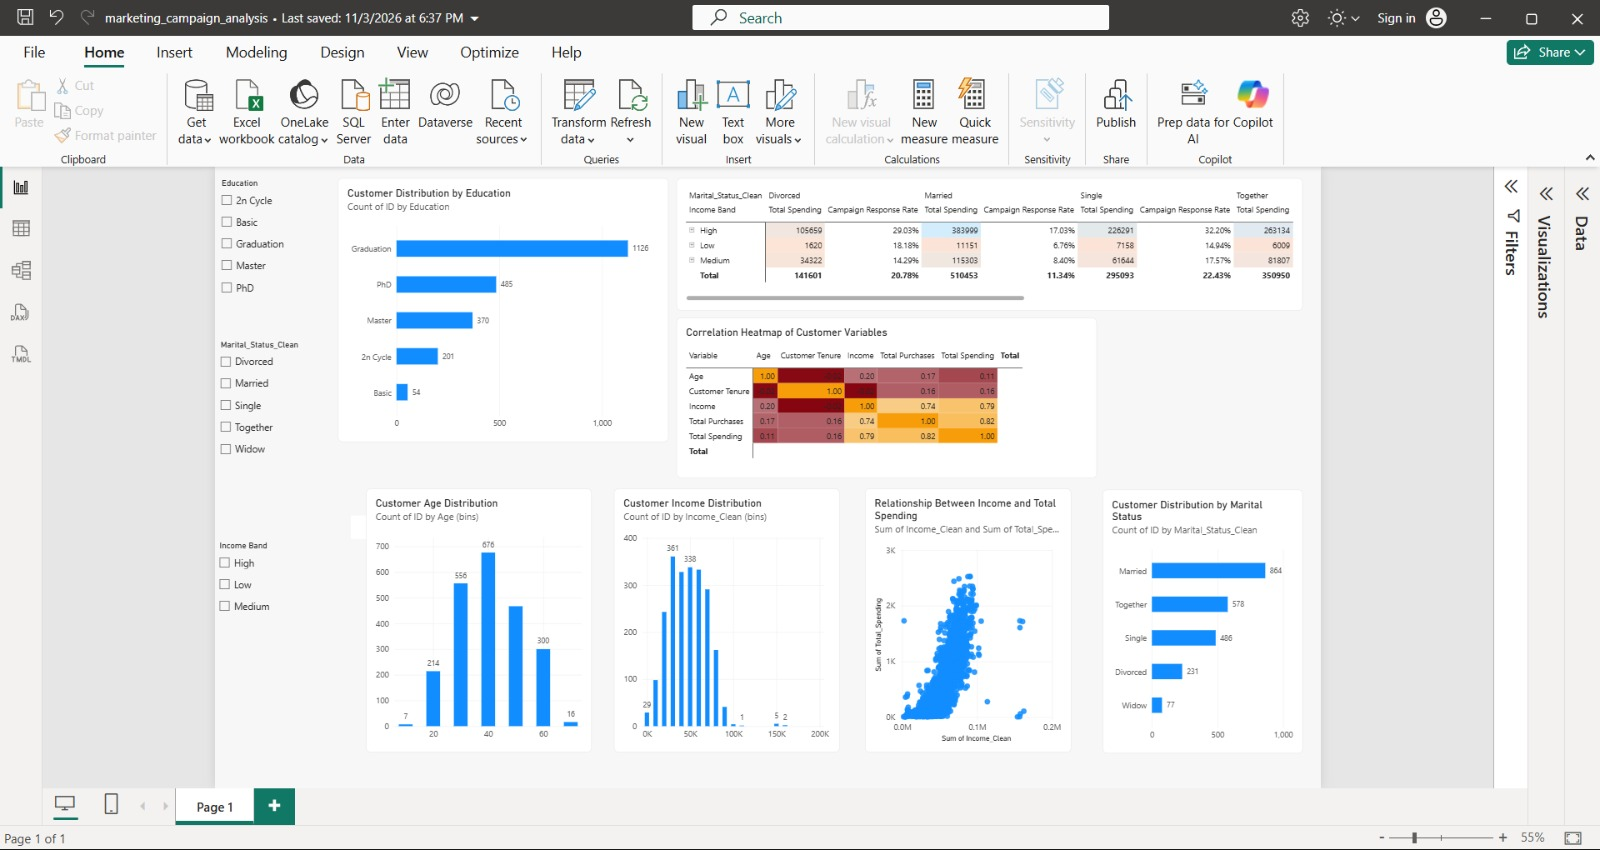
\includegraphics[width=\textwidth]{total-1.jpeg}
\caption{Complete PowerBI report page (slicers on the left; matrix scrolled to Divorced/Married/Single).}\label{fig:pbi-full}
\end{figure}
\begin{figure}[H]\centering
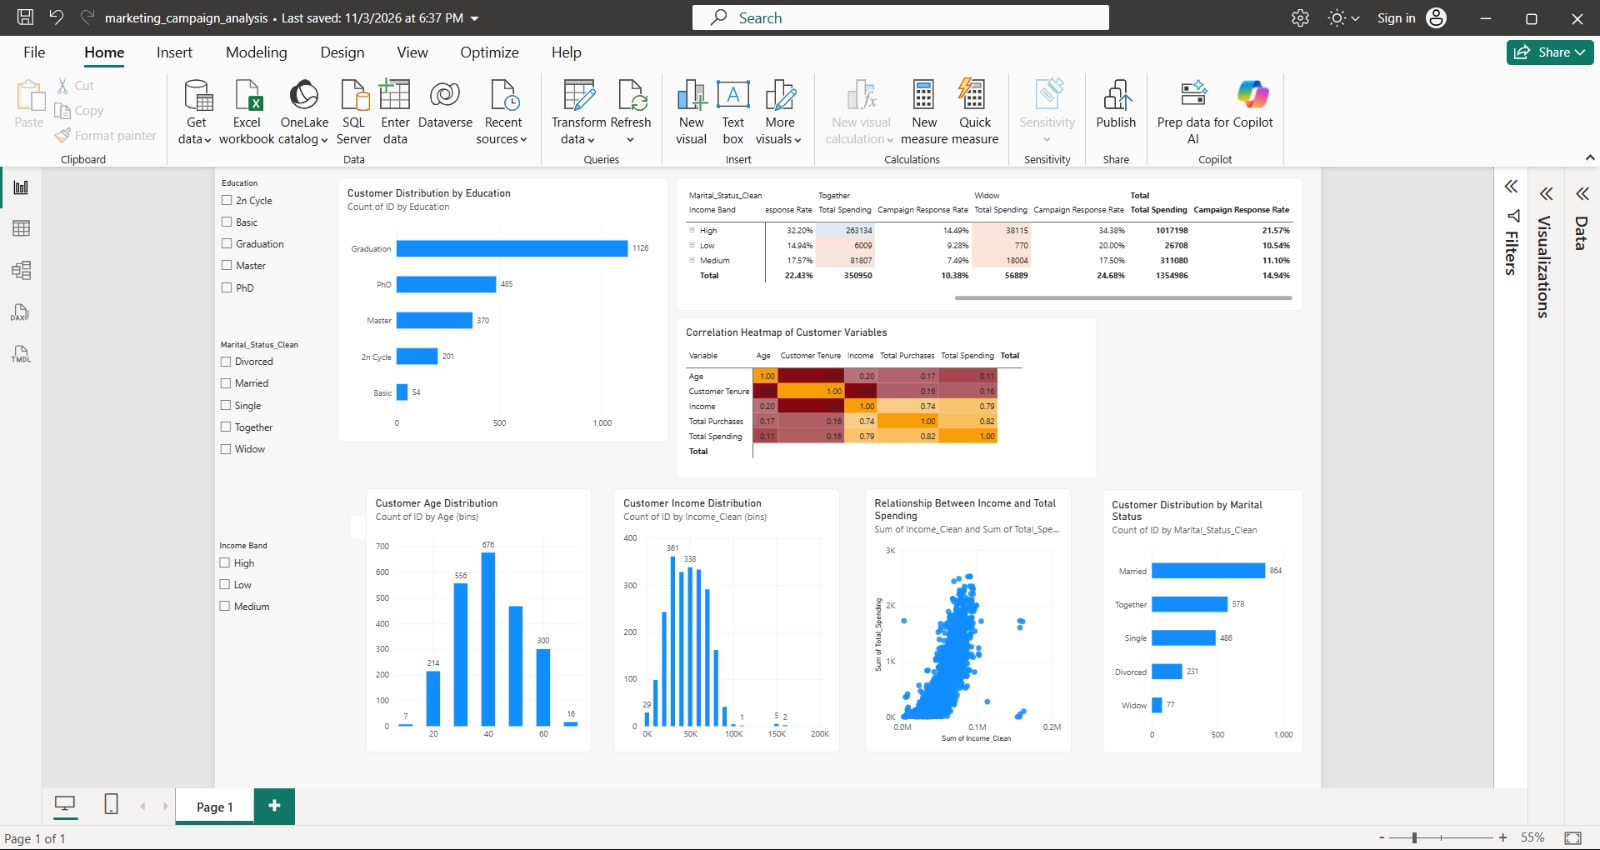
\includegraphics[width=\textwidth]{total-2.jpeg}
\caption{Same page with the matrix scrolled to Together/Widow and the grand totals.}
\end{figure}
\begin{figure}[H]\centering
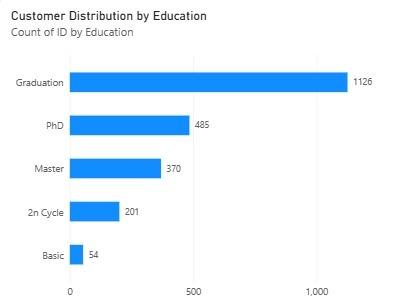
\includegraphics[height=5.2cm]{customerdistribution_education.jpeg}\hfill
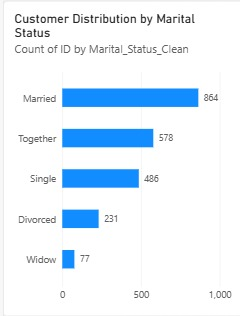
\includegraphics[height=5.2cm]{customerdistribution_maritialstatus.jpeg}
\caption{Bar charts: customers by Education and by Marital Status (after cleaning).}\label{fig:pbi-cat}
\end{figure}
\begin{figure}[H]\centering
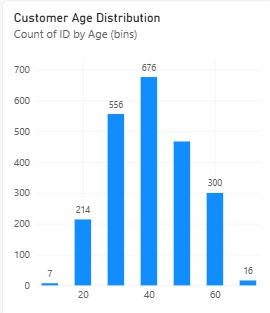
\includegraphics[height=5.2cm]{customer_age.jpeg}\hfill
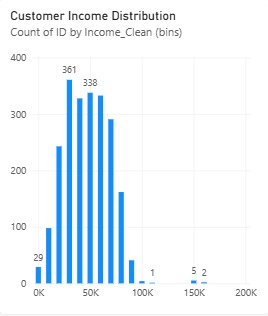
\includegraphics[height=5.2cm]{customer_income.jpeg}
\caption{Histograms of Age and Income\_Clean.}\label{fig:pbi-num}
\end{figure}
\begin{figure}[H]\centering
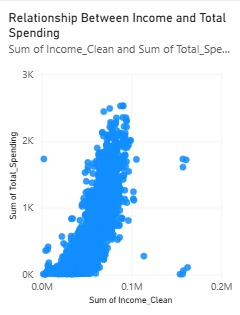
\includegraphics[height=5.5cm]{income_total_spending.jpeg}\hfill
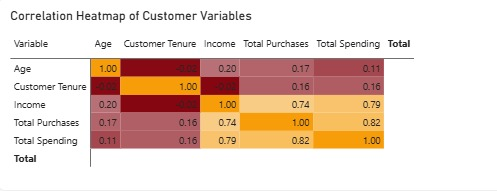
\includegraphics[height=4.6cm]{heatmap.jpeg}
\caption{Scatter plot of Income vs.\ Total Spending, and the correlation heatmap.}\label{fig:pbi-rel}
\end{figure}

\paragraph{What the visuals show.} Graduation is the largest education group (1{,}126), Basic
the smallest (54); Married (864) and Together (578) make up 65\% of customers. Age is roughly
bell-shaped (most customers 35--55). Income is right-skewed with a main mass of 20k--90k and a
few isolated values above 150k (kept, see Table~\ref{tab:pq}). The scatter shows a strong,
curved positive relationship between income and spending with near-zero spending below
$\approx$30k; the few points far to the right with very low spending are the high-income outliers.
In the heatmap, Total Spending correlates strongly with Total Purchases (0.82) and Income (0.79);
Age and Customer Tenure are almost uncorrelated with everything ($|r|\le0.20$).

\subsection{Quantified insights}
All values below refer to the 2{,}236 cleaned customers (overall response rate to the last
campaign 14.9\%, 334 responders; mean spending 606, median 396.5).
\begin{enumerate}
\item \textbf{Income drives spending.} Pearson $r(\text{Income},\text{Total Spending}) = 0.79$.
Mean spending rises from 72 ($<$30k, $n=370$) to 189 (30--50k), 746 (50--70k), 1{,}352
(70--90k) and 1{,}604 (90k+, $n=53$). The High band ($\ge$60k, 38\% of customers) generates 75\% of total
spending (1{,}017{,}198 of 1{,}354{,}986), the Low band only 2\%. \emph{Implication:} income is the first targeting
criterion for premium products; low-income customers need low-price offers.
\item \textbf{Spending is concentrated.} The top 20\% of customers generate 52.3\% of total
spending; wine (50.2\%) and meat (27.6\%) make up 78\% of revenue. \emph{Implication:}
retention of the top quintile and the wine/meat assortment matter most.
\item \textbf{Children reduce spending and response.} Customers without children spend 1{,}105
on average and respond at 26.5\%, versus 474 / 10.3\% with one child and 246 / 11.2\% with two
($r = -0.50$). Families buy more on deals (3.6 deal purchases with two children vs.\ 1.1 without).
\emph{Implication:} premium campaigns go to child-free households; families respond to discounts.
\item \textbf{Response rate rises sharply with income.} 10--12\% below 70k, 25.6\% at 70--90k
and 49.1\% at 90k+ (PowerBI matrix: High band 21.57\% vs.\ 11.10\% Medium and 10.54\% Low; highest
cell High~$\times$~Widow 34.4\%, lowest High~$\times$~Married 17.0\%). \emph{Implication:} the same
campaign is about five times as effective in the top band; untargeted mailing wastes contacts.
\item \textbf{Marital status and education matter.} Response is 22.4\% for Single, 20.8\%
Divorced and 24.7\% Widow, versus 11.3\% Married and 10.4\% Together. By education it rises
from 3.7\% (Basic, $n=54$) to 20.8\% (PhD). \emph{Implication:} single-person households and
highly educated customers are the most receptive audience (with an ethics check on using such
attributes).
\item \textbf{Web visits signal low value, not engagement.} Web visits correlate negatively with
spending ($r=-0.50$) and income ($r=-0.65$); customers with $\ge 7$ visits/month ($n=830$) spend
317 vs.\ 777 for the rest. \emph{Implication:} heavy browsers are price-sensitive; the website
needs conversion features (e.g.\ entry-level offers), not more traffic.
\item \textbf{Longer tenure, higher response.} Response is 8.6\% for the newest third of
customers (tenure $\le 244$ days), 11.9\% in the middle (245--470) and 24.3\% for the oldest third.
\emph{Implication:} loyal long-term customers should be prioritised; new customers need
onboarding before they respond to campaigns.
\end{enumerate}

%=====================================================================
\section{Task 2: K-Means Clustering from Scratch}
%=====================================================================
\subsection{Implementation}
\texttt{KMeansCustom} (Part2 notebook, NumPy only) contains:
\begin{itemize}
\item \textbf{k-means++ initialisation}: first centre uniformly at random; each further centre is
drawn with probability $\propto D(x)^2$, the squared distance to the nearest chosen centre.
\item \textbf{Lloyd iterations}: vectorised squared-Euclidean assignment, centroid update as the
mean of the members.
\item \textbf{Convergence}: stop when the largest centroid shift
$\max_j\lVert c_j^{new}-c_j^{old}\rVert_2 < 10^{-4}$, or after 300 iterations.
\item \textbf{Empty clusters}: an empty cluster's centre is moved to the point farthest from its
nearest centre (distinct points if several clusters are empty), i.e.\ to the worst-served region.
\item \textbf{Restarts}: \texttt{n\_init} independent runs with different seeds; the run with the
lowest inertia is kept.
\end{itemize}

\paragraph{Verification against sklearn.} With $k=4$, \texttt{n\_init}=15 and the same tolerance:
\begin{table}[H]\centering\small
\caption{Custom implementation vs.\ \texttt{sklearn.cluster.KMeans} ($k=4$).}
\begin{tabular}{@{}lr@{}}\toprule
Quantity & Value\\\midrule
Custom inertia (22 iterations) & 9{,}798.13\\
sklearn inertia (22 iterations) & 9{,}798.00\\
Ratio custom/sklearn & 1.000014 (0.0014\% difference)\\
ARI between labelings (independent inits) & 0.946\\
ARI / inertia when sklearn starts from our final centroids & 1.000 / 9{,}798.13\\\bottomrule
\end{tabular}\end{table}
The independent runs reach two nearly equal local optima that differ only in a few boundary
customers (ARI 0.946). Started from our centroids, sklearn reproduces our labelling exactly,
so the assignment, update and convergence steps are equivalent.

\subsection{Feature choice and scaling}
{\sloppy Eight numerical features describing value, life stage and engagement are used:
\texttt{Age}, \texttt{Income\_Clean}, \texttt{Total\_Spending}, \texttt{Total\_Purchases},
\texttt{Total\_Children}, \texttt{Customer\_Tenure}, \texttt{Recency}, \texttt{NumWebVisitsMonth}.
Excluded are \texttt{Response}, \texttt{AcceptedCmp1--5} (reserved for Section 3), identifiers and
raw columns replaced by derived ones (\texttt{ID}, \texttt{Year\_Birth}, raw \texttt{Income} with 24
NaNs, \texttt{Income\_Imputed}), the individual \texttt{Mnt*}/\texttt{Num*Purchases} columns (summarised
by the totals and used only for profiling), the constants \texttt{Z\_*}, and the categorical
\texttt{Education}, \texttt{Marital\_Status} and \texttt{Complain}, which are held out for external validation.
All features are standardised (zero mean, unit variance).\par}

\paragraph{Why unscaled or one-hot features are problematic.} K-Means minimises squared
Euclidean distance, so each feature's weight equals its variance. Unscaled, \texttt{Income\_Clean}
(std 21{,}411) contributes squared differences of order $10^9$ while \texttt{Total\_Children}
(0--3) contributes at most 9: the clustering would just be income bands. One-hot columns are
binary, each contributing 0 or 1; their effective weight depends on the number of categories and
their frequencies, not on importance, and the ``mean'' of dummies is not a category, so centroids
are hard to interpret. Moreover distances between categories are all equal, which K-Means cannot
exploit meaningfully; mixed data would need k-prototypes or Gower distance instead.

\subsection{\texorpdfstring{Choosing $k$}{Choosing k}}
The implementation was run for $k=2,\dots,10$ (\texttt{n\_init}=15). Stability is measured as the
mean pairwise ARI over 12 seeds and as the ARI of 50 bootstrap fits against the full-data labels.

\begin{figure}[H]\centering
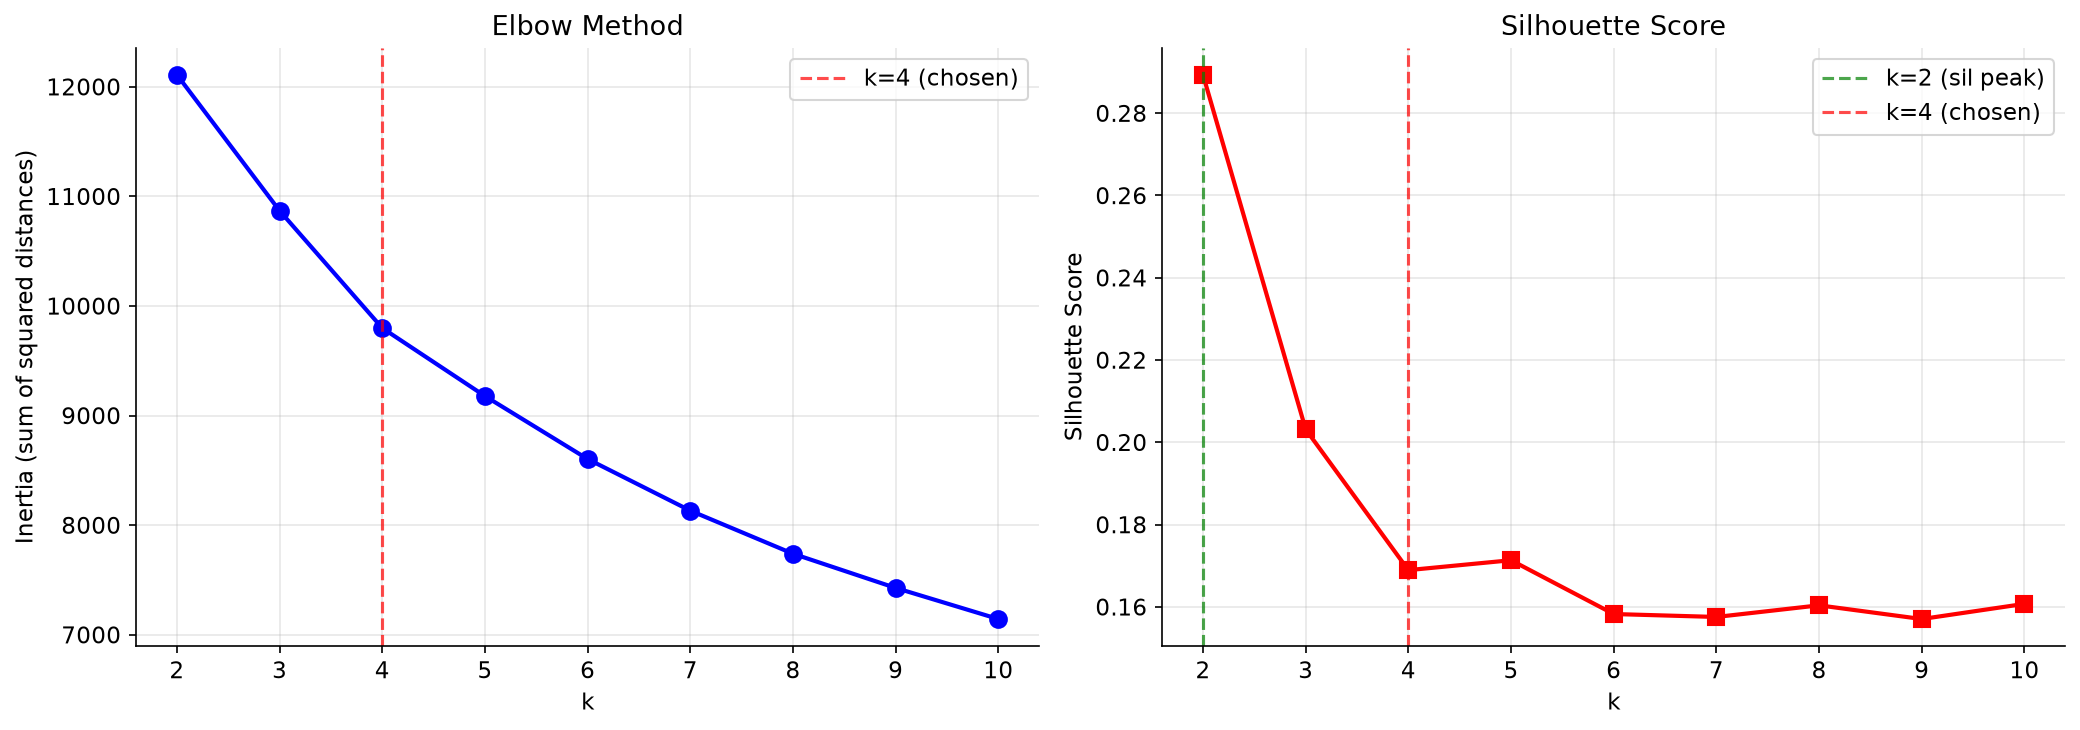
\includegraphics[width=\textwidth]{kmeans_k_selection.png}
\caption{Elbow (inertia) and silhouette for $k=2..10$.}\label{fig:ksel}
\end{figure}
\begin{figure}[H]\centering
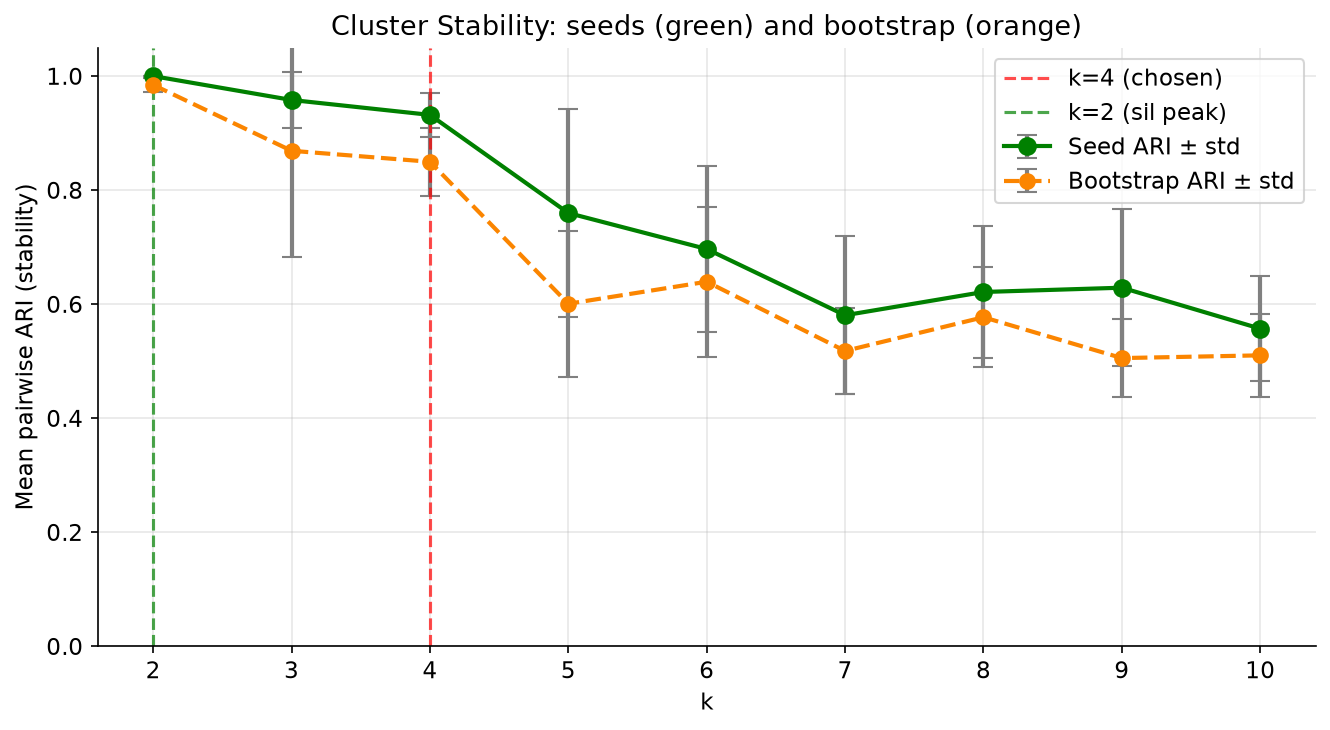
\includegraphics[width=0.62\textwidth]{kmeans_stability.png}
\caption{Seed and bootstrap stability (ARI $\pm$ std) by $k$.}\label{fig:stab}
\end{figure}

\begin{table}[H]\centering\small
\caption{Model-selection criteria for $k=2..10$ (chosen $k=4$ in bold).}\label{tab:ksel}
\begin{tabular}{@{}rrrrrr@{}}\toprule
$k$ & Inertia & $\Delta$Inertia (\%) & Silhouette & Seed ARI ($\pm$sd) & Bootstrap ARI ($\pm$sd)\\\midrule
2 & 12{,}108.89 & -- & 0.2893 & 1.000 (0.000) & 0.985 (0.012)\\
3 & 10{,}868.44 & 10.2 & 0.2031 & 0.958 (0.049) & 0.869 (0.186)\\
\textbf{4} & \textbf{9{,}798.13} & \textbf{9.8} & \textbf{0.1689} & \textbf{0.932 (0.039)} & \textbf{0.850 (0.060)}\\
5 & 9{,}177.56 & 6.3 & 0.1713 & 0.760 (0.183) & 0.601 (0.128)\\
6 & 8{,}603.06 & 6.3 & 0.1583 & 0.697 (0.145) & 0.639 (0.131)\\
7 & 8{,}132.02 & 5.5 & 0.1575 & 0.581 (0.138) & 0.518 (0.075)\\
8 & 7{,}739.09 & 4.8 & 0.1604 & 0.621 (0.116) & 0.577 (0.088)\\
9 & 7{,}426.77 & 4.0 & 0.1570 & 0.629 (0.138) & 0.505 (0.068)\\
10 & 7{,}143.07 & 3.8 & 0.1607 & 0.557 (0.092) & 0.510 (0.073)\\\bottomrule
\end{tabular}\end{table}

\begin{itemize}
\item \textbf{Elbow}: weak; the relative drop is 10.2\% and 9.8\% up to $k=4$ and then 6.3\% or
less, i.e.\ only a mild bend at $k=4$.
\item \textbf{Silhouette}: peaks at $k=2$ (0.289) and is flat at 0.16--0.17 for $k\ge4$. All values
are low: customer data forms overlapping groups rather than separated blobs.
\item \textbf{Stability}: high up to $k=4$ (seed 0.932, bootstrap 0.850 with small spread), then a
sharp drop at $k=5$ (0.760 / 0.601). $k=3$ has a slightly higher bootstrap mean (0.869) but three
times the spread (0.186), so it is less consistent.
\end{itemize}
\textbf{Decision: $k=4$}, the largest stable $k$; higher $k$ buys no silhouette but costs stability.
\textbf{Business usability:} $k=2$ is just ``rich/high-spend vs.\ poor/low-spend'', too coarse for
differentiated campaigns. Four segments are few enough that a marketing team can design and run one
campaign per segment, and (Section~\ref{sec:profiles}) they differ interpretably in income,
spending, family, tenure and channel. More than $\approx$6 segments would be unstable and
hard to operationalise.

\subsection{Cluster profiles and personas}\label{sec:profiles}
Final model: $k=4$, \texttt{n\_init}=20; sizes 592 / 530 / 518 / 596; silhouette 0.169,
Davies--Bouldin 1.88, Calinski--Harabasz 614.3.

\begin{table}[H]\centering
\caption{Cluster means in original units (the last four columns were not used for clustering).}\label{tab:profile}
\resizebox{\textwidth}{!}{%
\begin{tabular}{@{}lrrrrrrrrrrrrr@{}}\toprule
Cl. & $n$ & Age & Income & Spend & Purch. & Children & Tenure (d) & Recency & Web visits & Web p. & Cat.\ p. & Store p. & Deals\\\midrule
0 & 592 & 36.7 & 29{,}470 & 113 & 6.1 & 0.96 & 419 & 46.5 & 7.32 & 2.40 & 0.54 & 3.18 & 2.18\\
1 & 530 & 45.5 & 77{,}349 & 1{,}323 & 19.0 & 0.16 & 302 & 48.8 & 2.29 & 4.88 & 5.83 & 8.32 & 1.16\\
2 & 518 & 49.3 & 61{,}038 & 944 & 19.0 & 1.03 & 483 & 49.4 & 5.89 & 6.73 & 3.92 & 8.31 & 3.51\\
3 & 596 & 49.5 & 43{,}804 & 164 & 7.6 & 1.58 & 223 & 51.8 & 5.53 & 2.77 & 0.87 & 3.96 & 2.48\\\midrule
All & 2{,}236 & 45.1 & 51{,}953 & 606 & 12.6 & 0.95 & 354 & 49.1 & 5.32 & 4.09 & 2.66 & 5.80 & 2.33\\\bottomrule
\end{tabular}}\end{table}

\begin{figure}[H]\centering
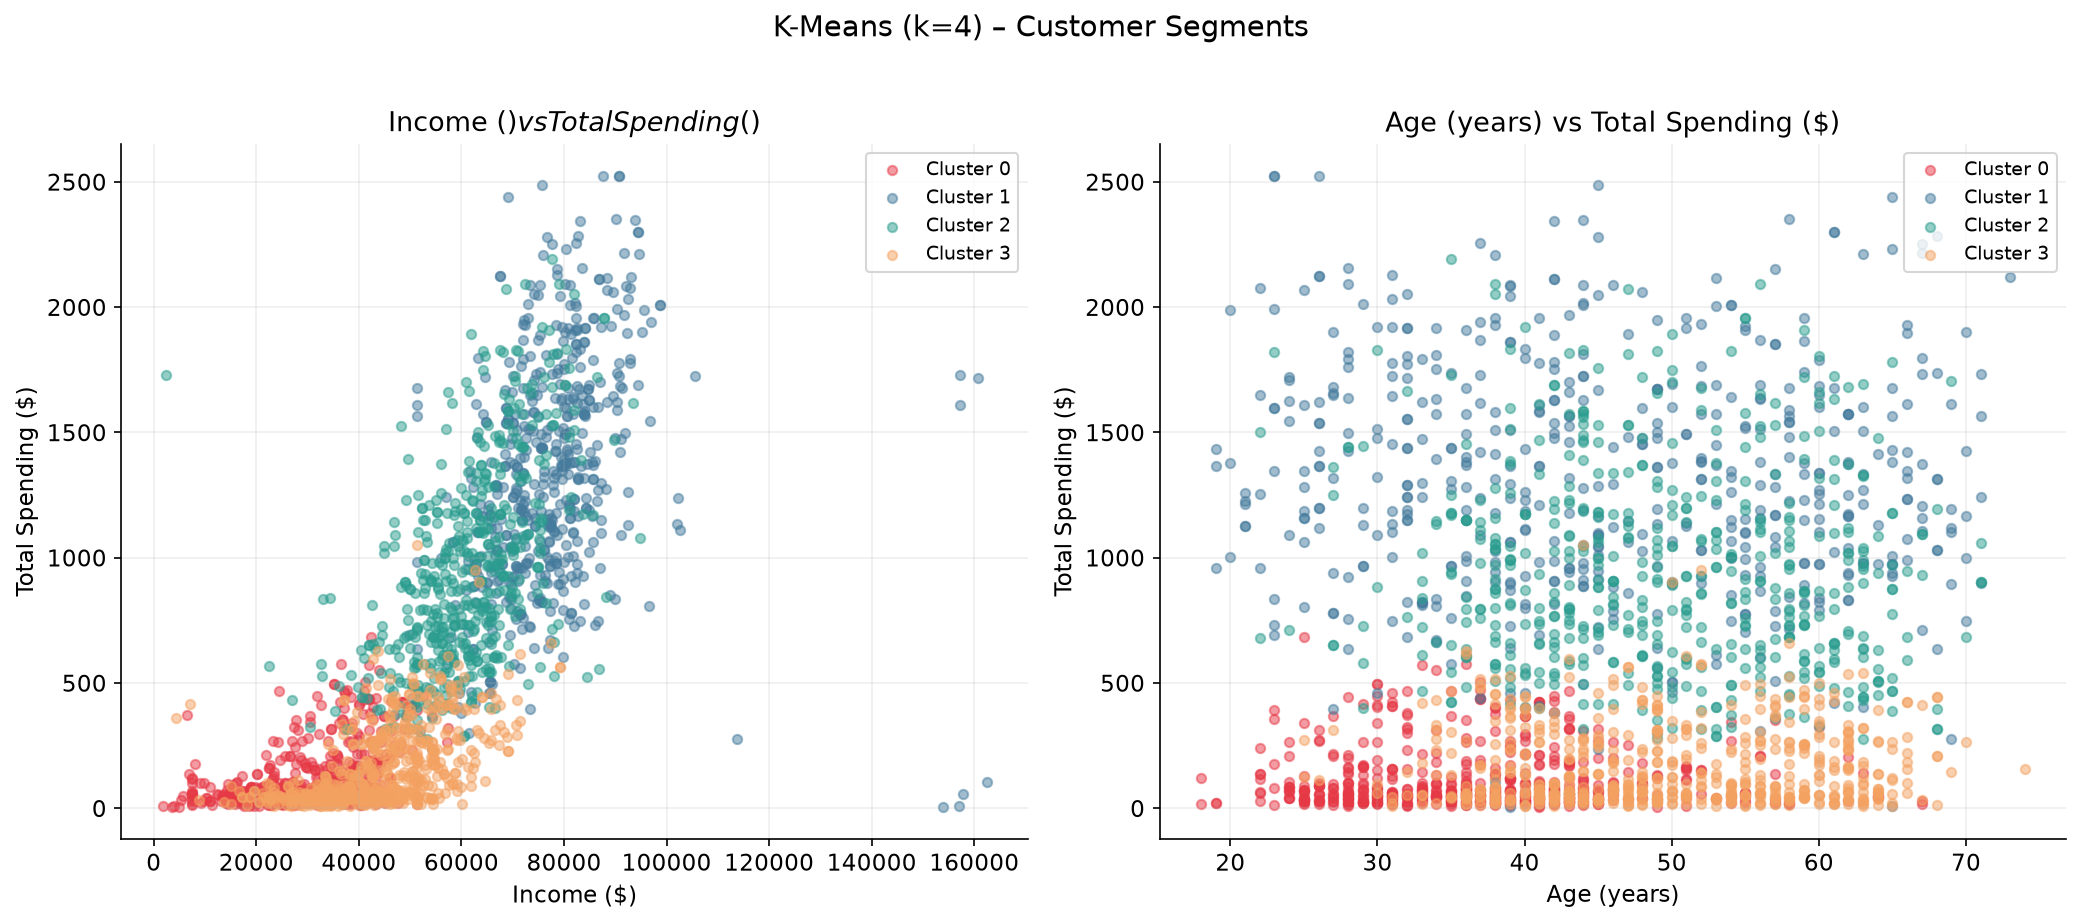
\includegraphics[width=\textwidth]{kmeans_clusters_scatter.png}
\caption{Clusters in Income vs.\ Total Spending and Age vs.\ Total Spending.}
\end{figure}
\begin{figure}[H]\centering
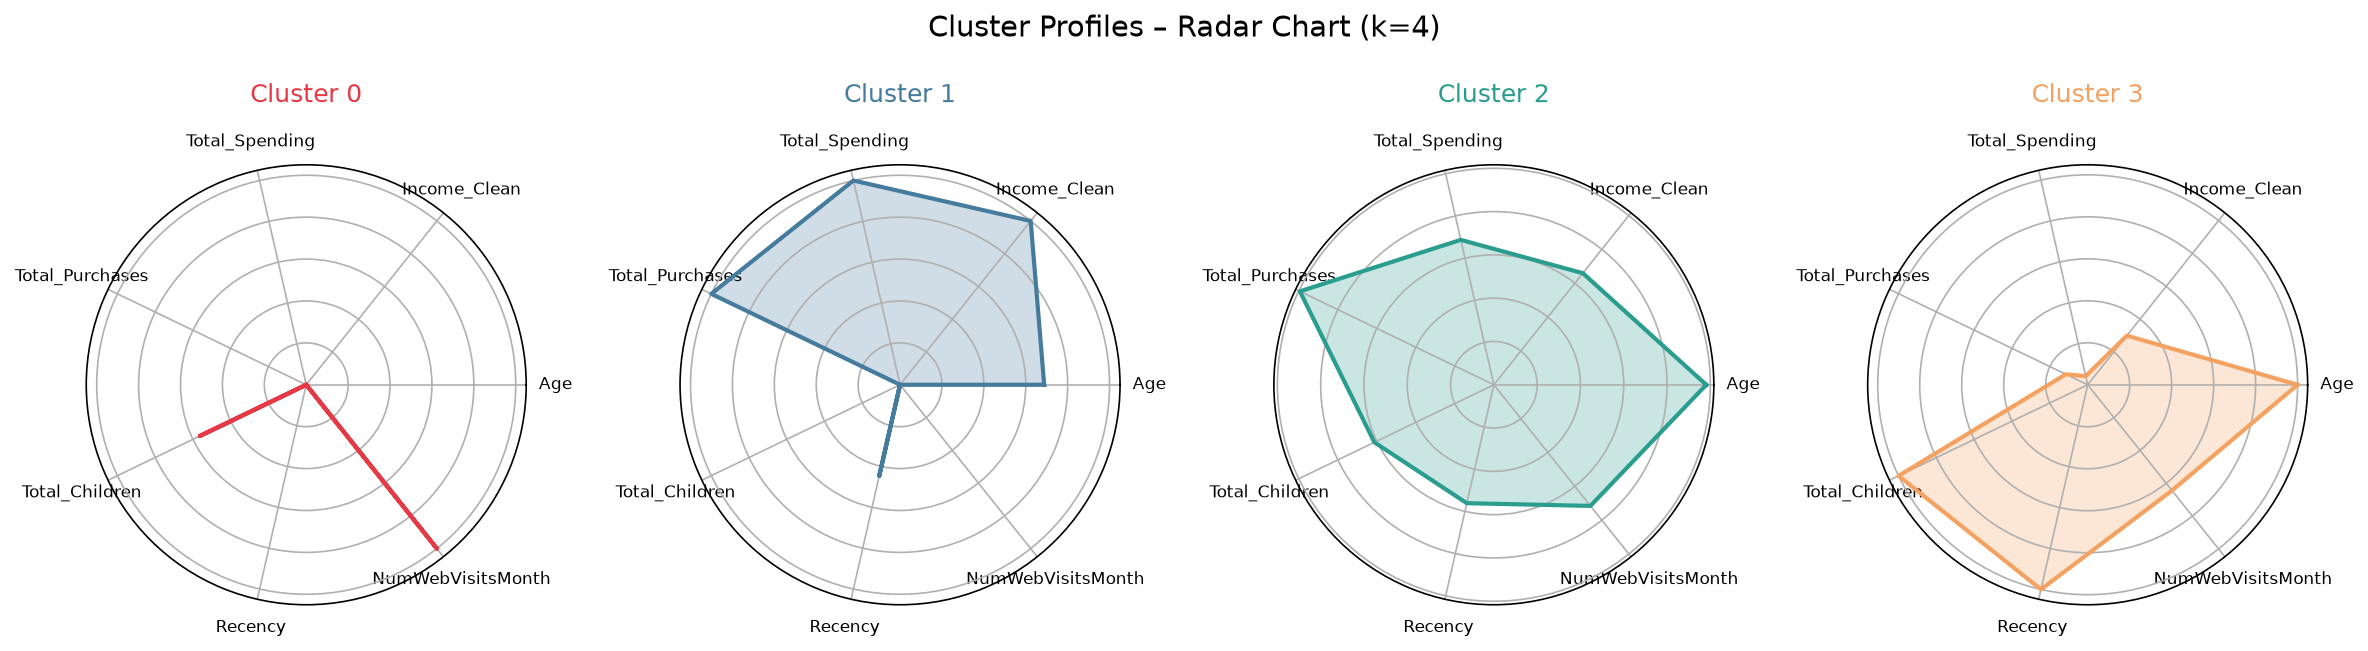
\includegraphics[width=\textwidth]{kmeans_radar_chart.png}
\caption{Normalised cluster profiles (radar charts).}
\end{figure}
\begin{figure}[H]\centering
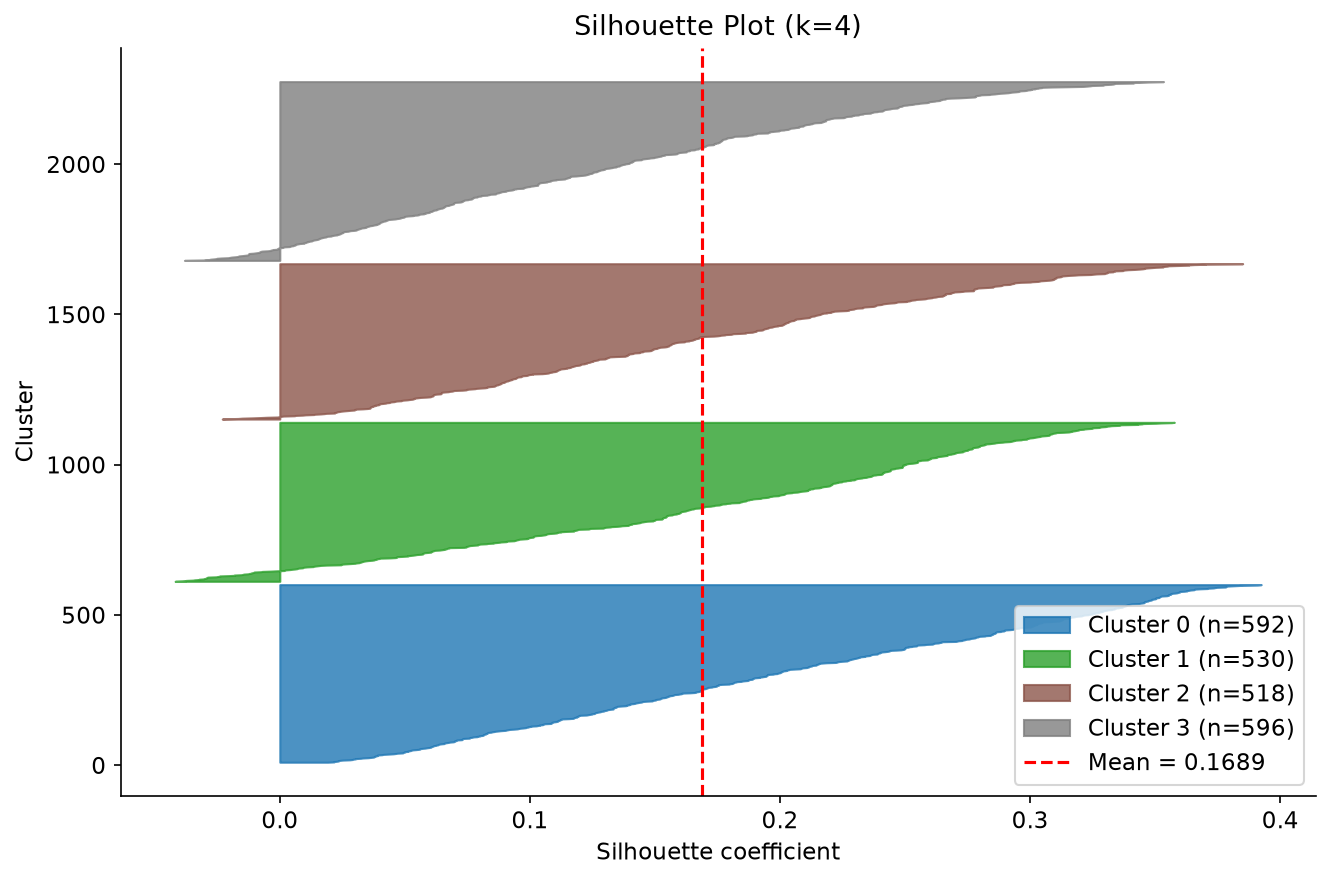
\includegraphics[width=0.55\textwidth]{silhouette_plot_final_k.png}
\caption{Silhouette plot for $k=4$: few negative values, but low average width (0.169).}
\end{figure}

\begin{description}
\item[Cluster 0 --- Young Budget Browsers (592).] Youngest (36.7) and lowest income (29{,}470),
lowest spending (113) and purchases (6.1), but the most web visits (7.3/month) with few web
purchases. \emph{Lever:} low-price entry offers and web conversion nudges.
\item[Cluster 1 --- Affluent Child-free Big Spenders (530).] Highest income (77{,}349) and spending
(1{,}323), almost no children (0.16), most catalogue purchases (5.8), fewest web visits (2.3) and
deal purchases (1.2). \emph{Lever:} premium catalogue/in-store offers; discounts unnecessary.
\item[Cluster 2 --- Loyal Multichannel Deal-Seekers (518).] Upper-middle income (61{,}038), high
spending (944), longest tenure (483 days), most web (6.7) and deal (3.5) purchases.
\emph{Lever:} deal-based loyalty programme, cross-channel bundles.
\item[Cluster 3 --- New Budget Families (596).] Below-average income (43{,}804), low spending (164),
most children (1.58), shortest tenure (223 days). \emph{Lever:} onboarding and family value bundles.
\end{description}
Recency is nearly identical across clusters (46--52 days) and does not characterise any segment.

\subsection{External validation: Education and Complain}
Neither variable was used for clustering. For \emph{Complain} only 20 customers complained and 2 of
8 expected counts are below 5, so a Monte-Carlo permutation p-value (10{,}000 permutations) is
reported next to the asymptotic one; Cramér's $V=\sqrt{\chi^2/(n(\min(r,c)-1))}$ is given in its
standard and bias-corrected (Bergsma) form.

\begin{table}[H]\centering\small
\caption{$\chi^2$ tests of independence with the cluster labels.}\label{tab:chi}
\begin{tabular}{@{}lrrrrrr@{}}\toprule
Variable & $\chi^2$ & df & $p$ (asympt.) & $p$ (perm.) & $V$ & $V$ (bias-corr.)\\\midrule
Education & 172.15 & 12 & $1.7\times10^{-30}$ & $\le 10^{-4}$ & 0.160 & 0.155\\
Complain & 1.25 & 3 & 0.741 & 0.748 & 0.024 & 0.000\\\bottomrule
\end{tabular}\end{table}

\begin{figure}[H]\centering
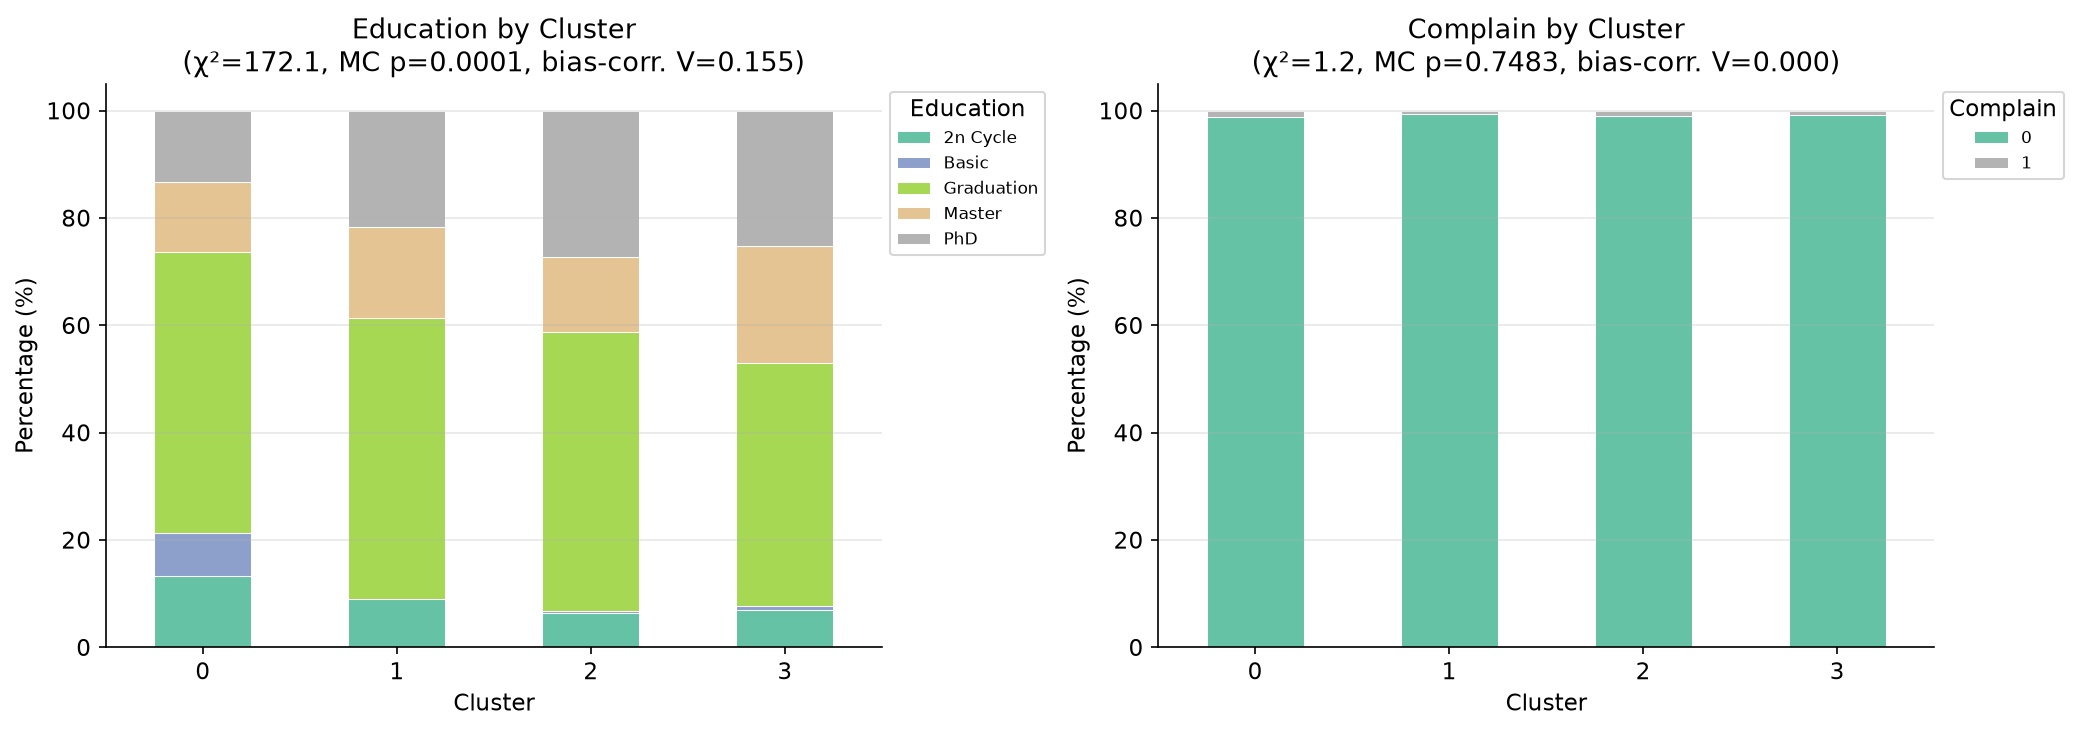
\includegraphics[width=\textwidth]{external_validation.png}
\caption{Education and Complain composition per cluster.}
\end{figure}
Education differs significantly but weakly ($V=0.16$): cluster 0 holds 47 of the 54 \emph{Basic}
customers (14.3 expected) and fewer PhDs than expected (79 vs.\ 128), clusters 2 and 3 more.
Complaints are spread uniformly across segments (not significant, $V\approx0$).

\paragraph{Why tests on clustering features prove nothing.} K-Means chooses the partition that
maximises the separation of cluster means on exactly those features. An ANOVA on, say,
\texttt{Income\_Clean} would give $p\approx0$ by construction---even on pure noise K-Means creates
groups with different means. The test's null hypothesis (group membership independent of the
feature) is violated by the procedure itself, so the p-value only confirms that the algorithm ran.
Only variables the algorithm never saw, such as Education and Complain, provide honest evidence.

%=====================================================================
\section{Task 3: Comparing Clustering Algorithms}
%=====================================================================
\subsection{Datasets and setup}
Dataset2 contains four 2-D sets (\texttt{x1}, \texttt{x2}), each standardised before clustering:
\emph{Compact} (400 points; five tight, equal circular blobs), \emph{Skewed} (925; one large diffuse
cloud and two small denser groups at its lower edge), \emph{Subclusters} (400; four groups, the
top-right one made of two adjacent sub-clusters), \emph{WellSeparated} (335; three round clusters
with clear gaps). K-Means and every agglomerative linkage choose $k\in[2,8]$ resp.\ $[2,10]$ by
maximum silhouette, independently per method.

\begin{figure}[H]\centering
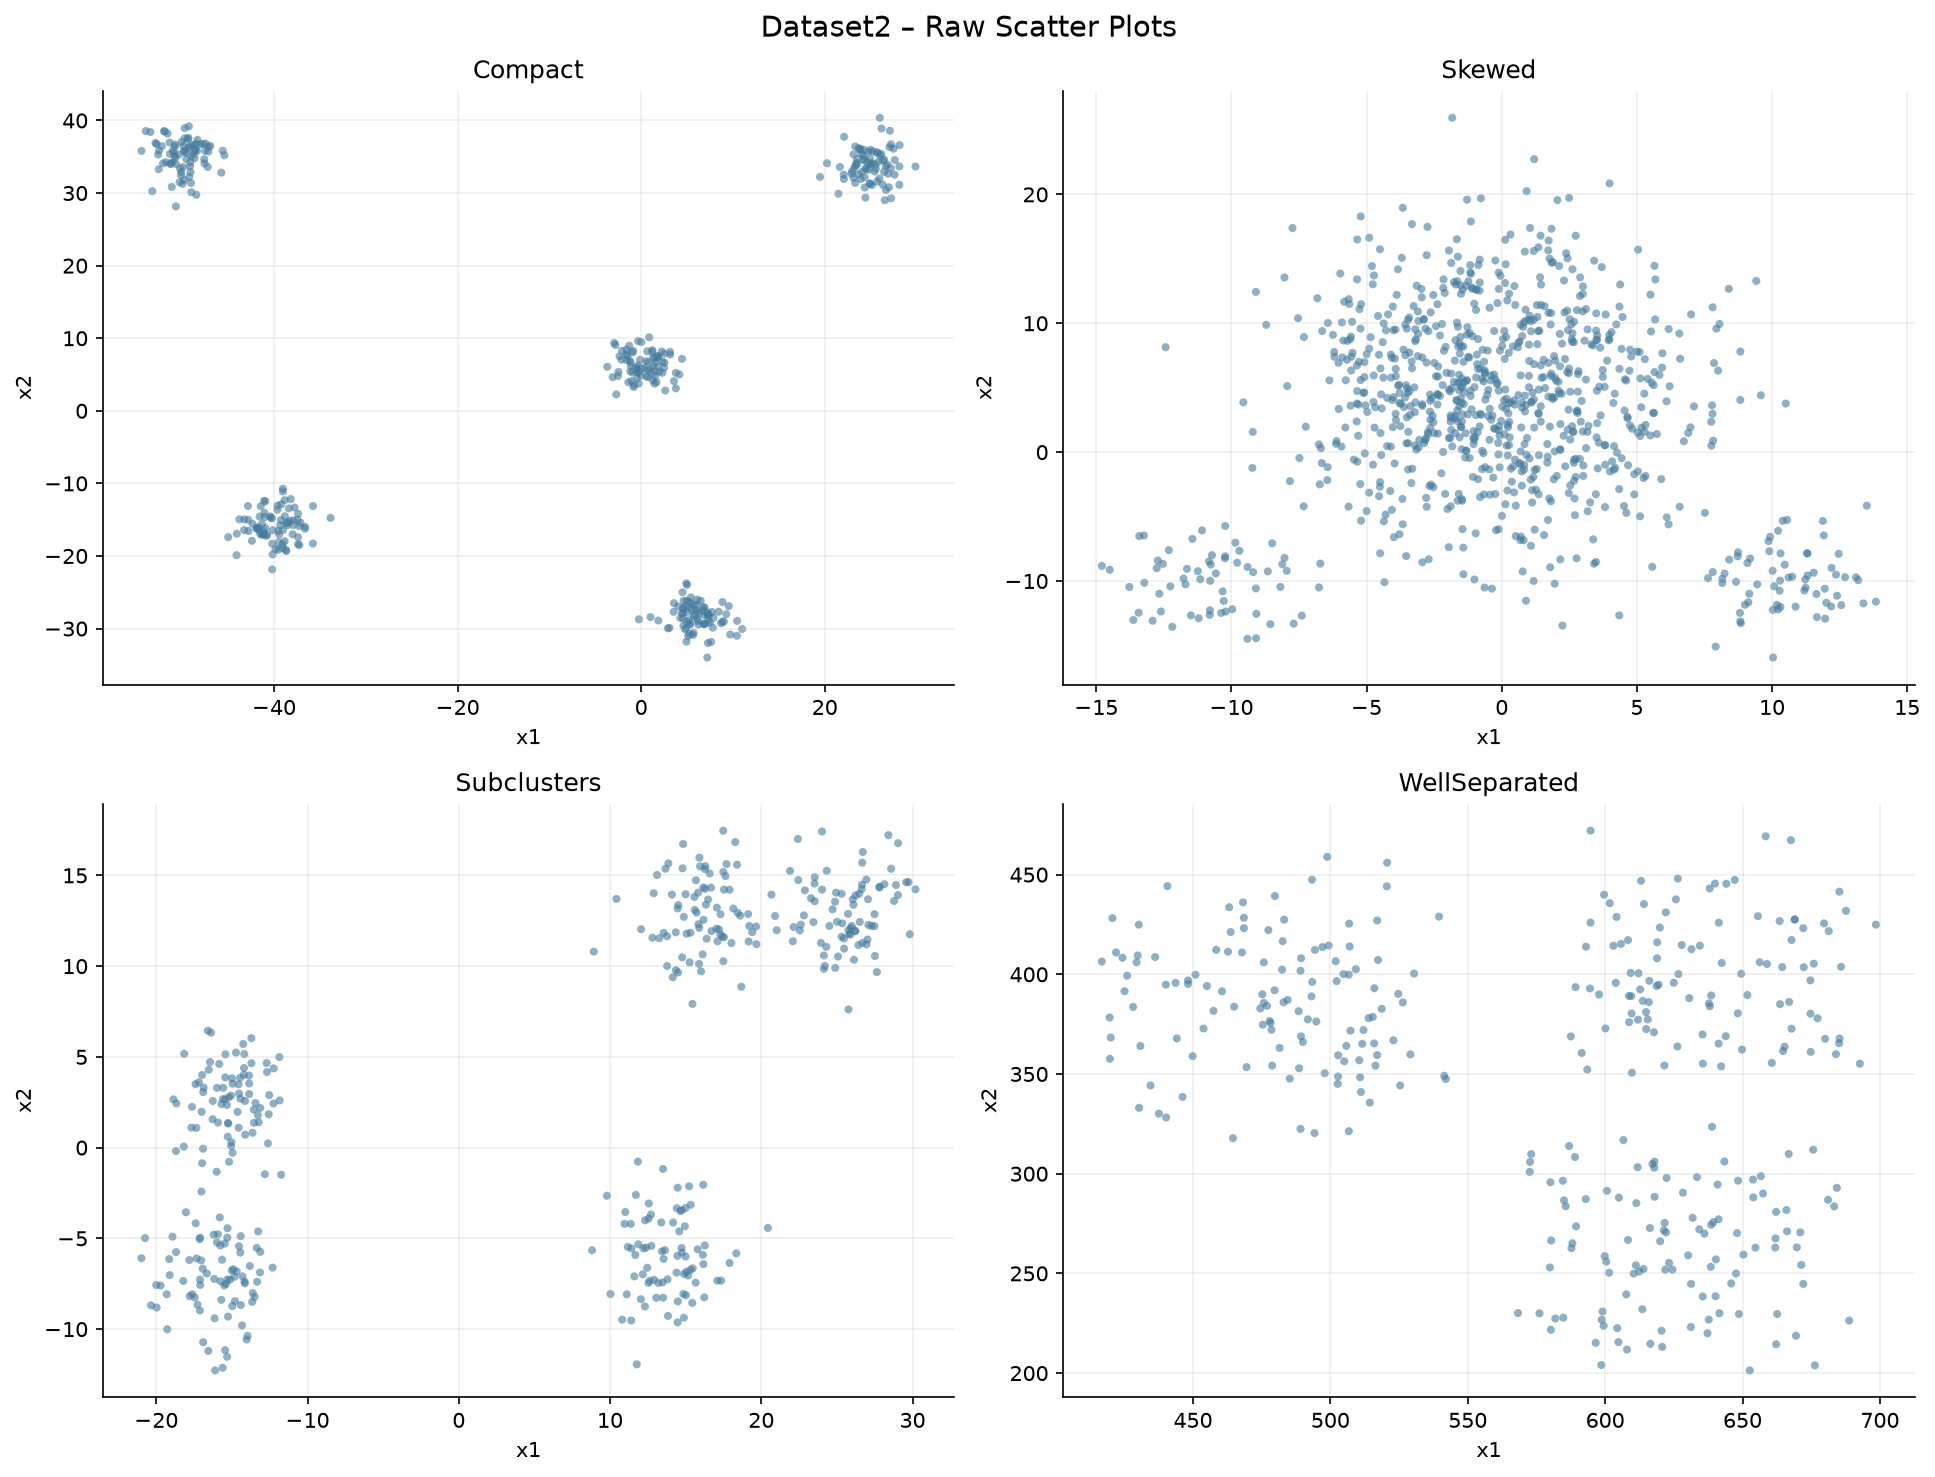
\includegraphics[width=0.62\textwidth]{part3_raw_datasets.png}
\caption{Raw Dataset2 point clouds.}
\end{figure}

\subsection{K-Means}
\begin{figure}[H]\centering
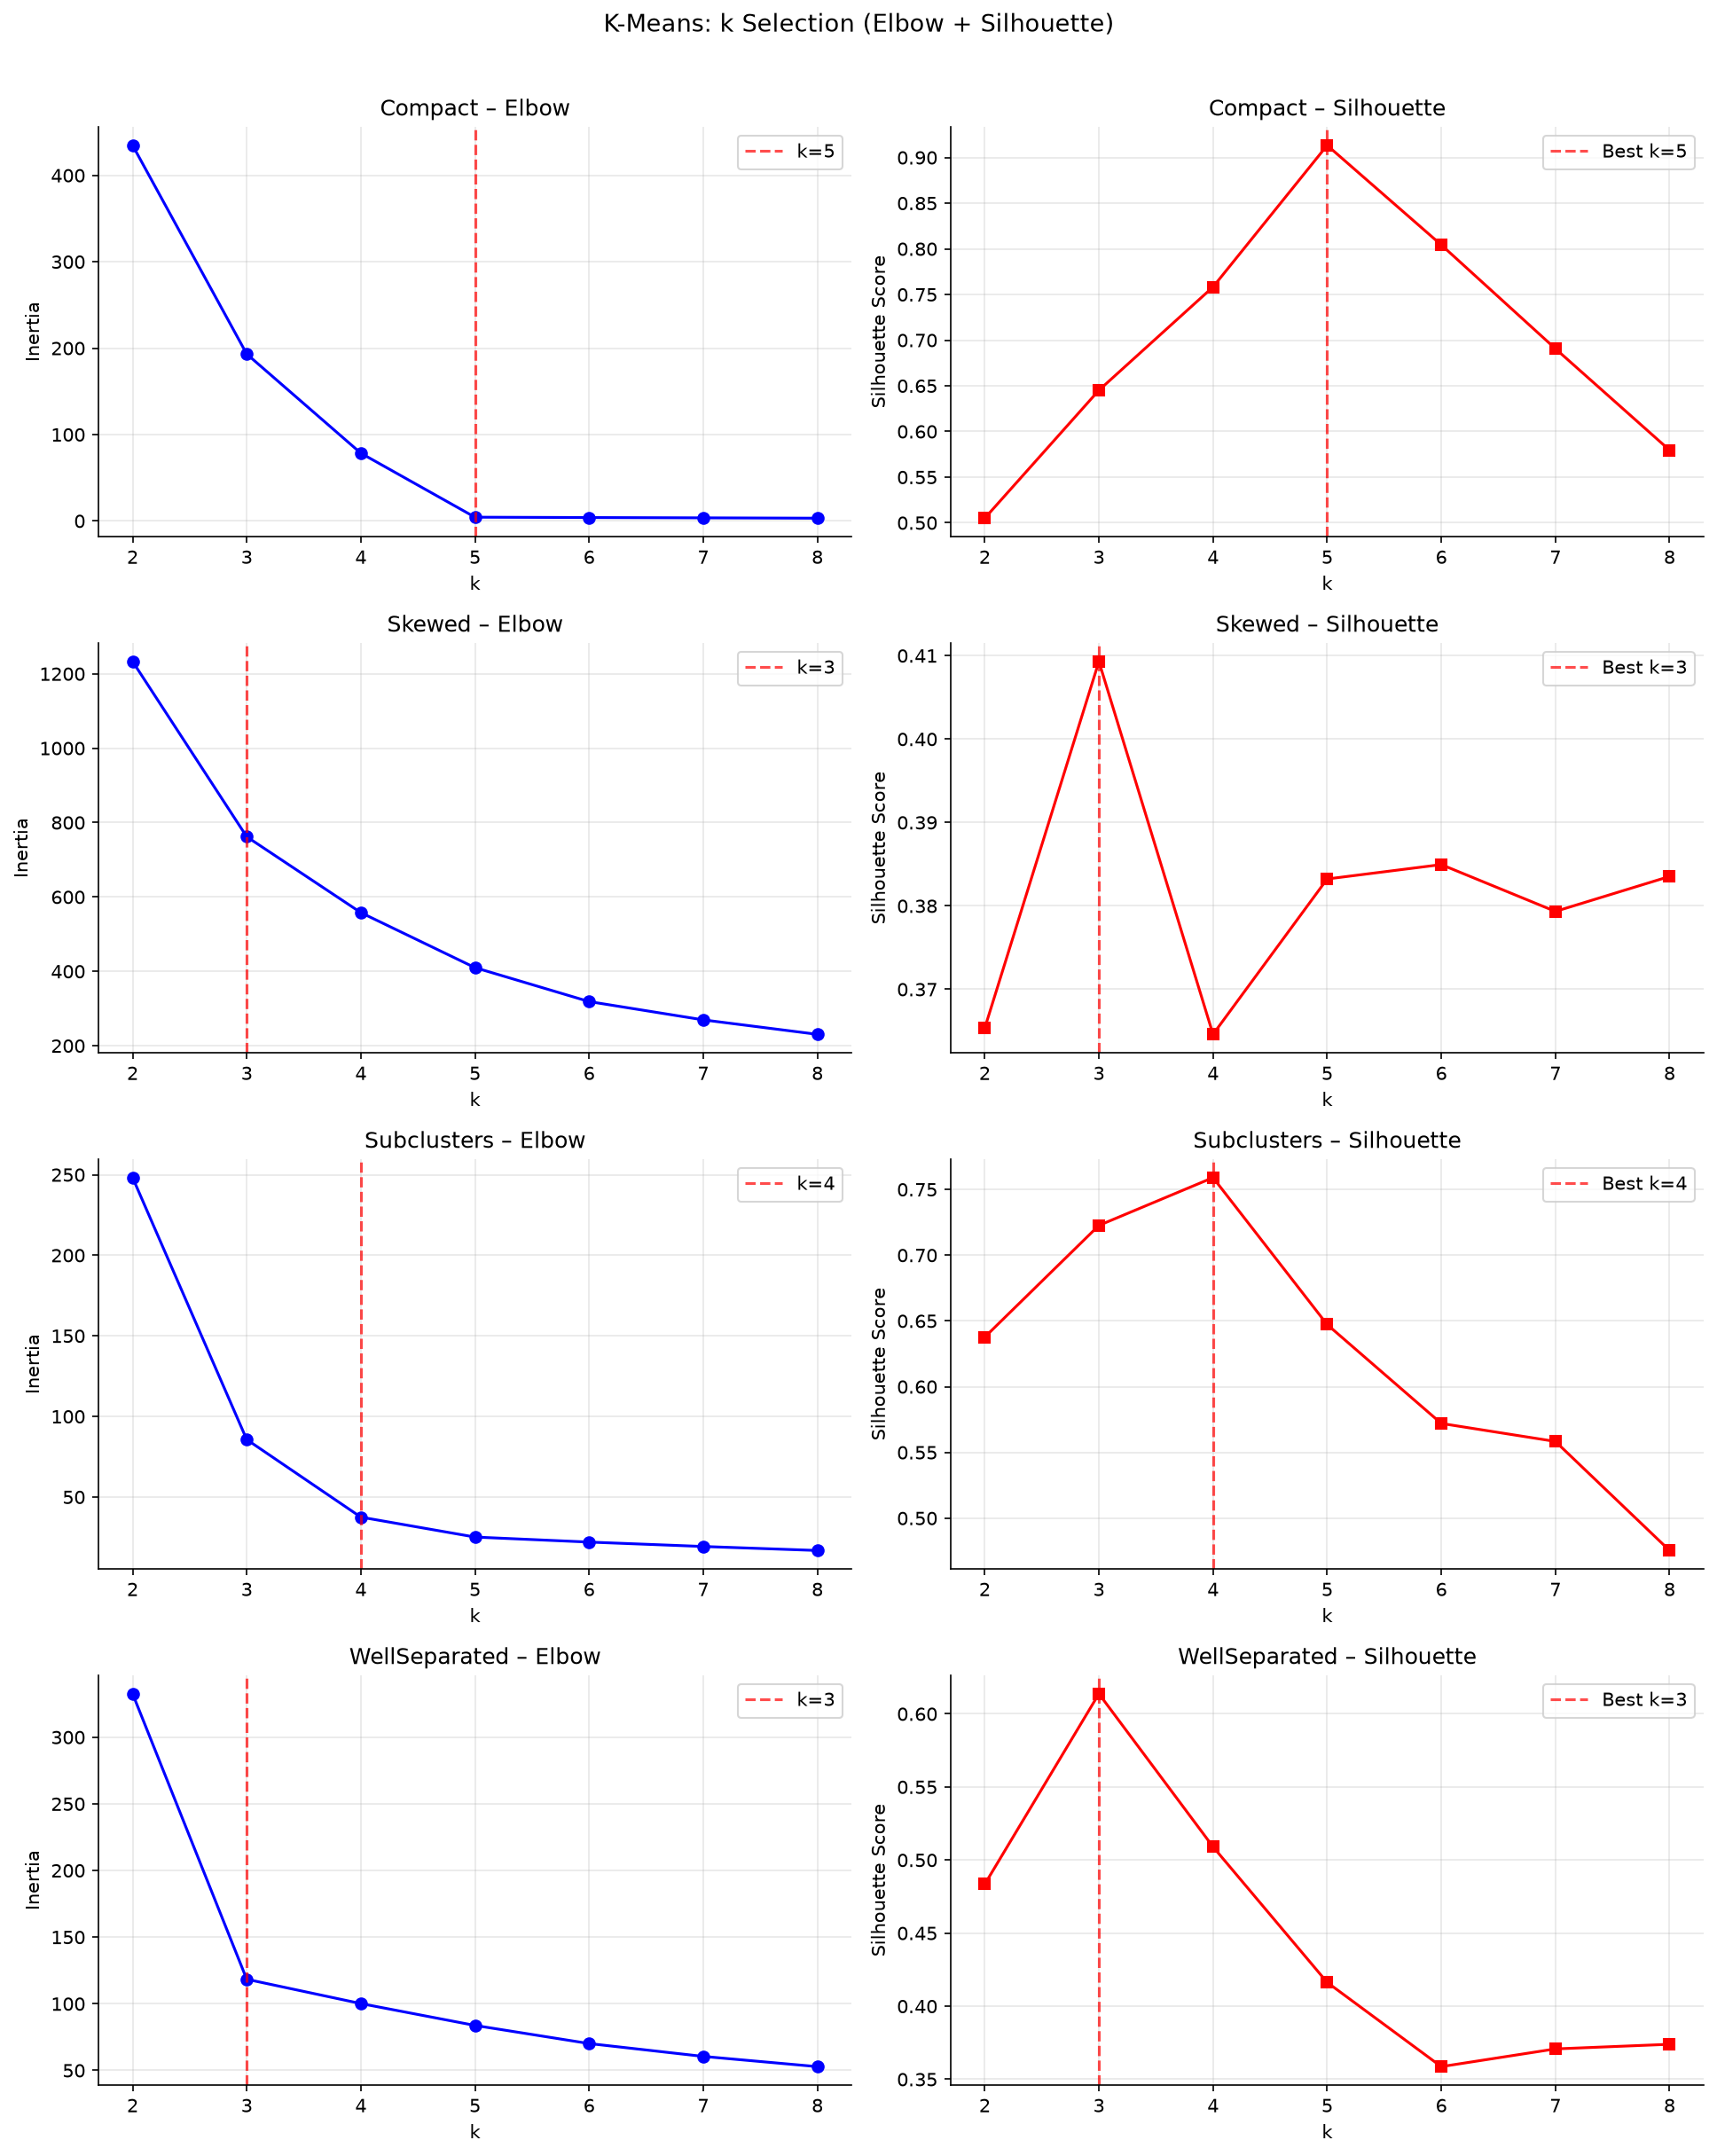
\includegraphics[width=0.55\textwidth]{part3_kmeans_k_selection.png}
\caption{Elbow and silhouette curves per dataset (K-Means).}
\end{figure}
\begin{figure}[H]\centering
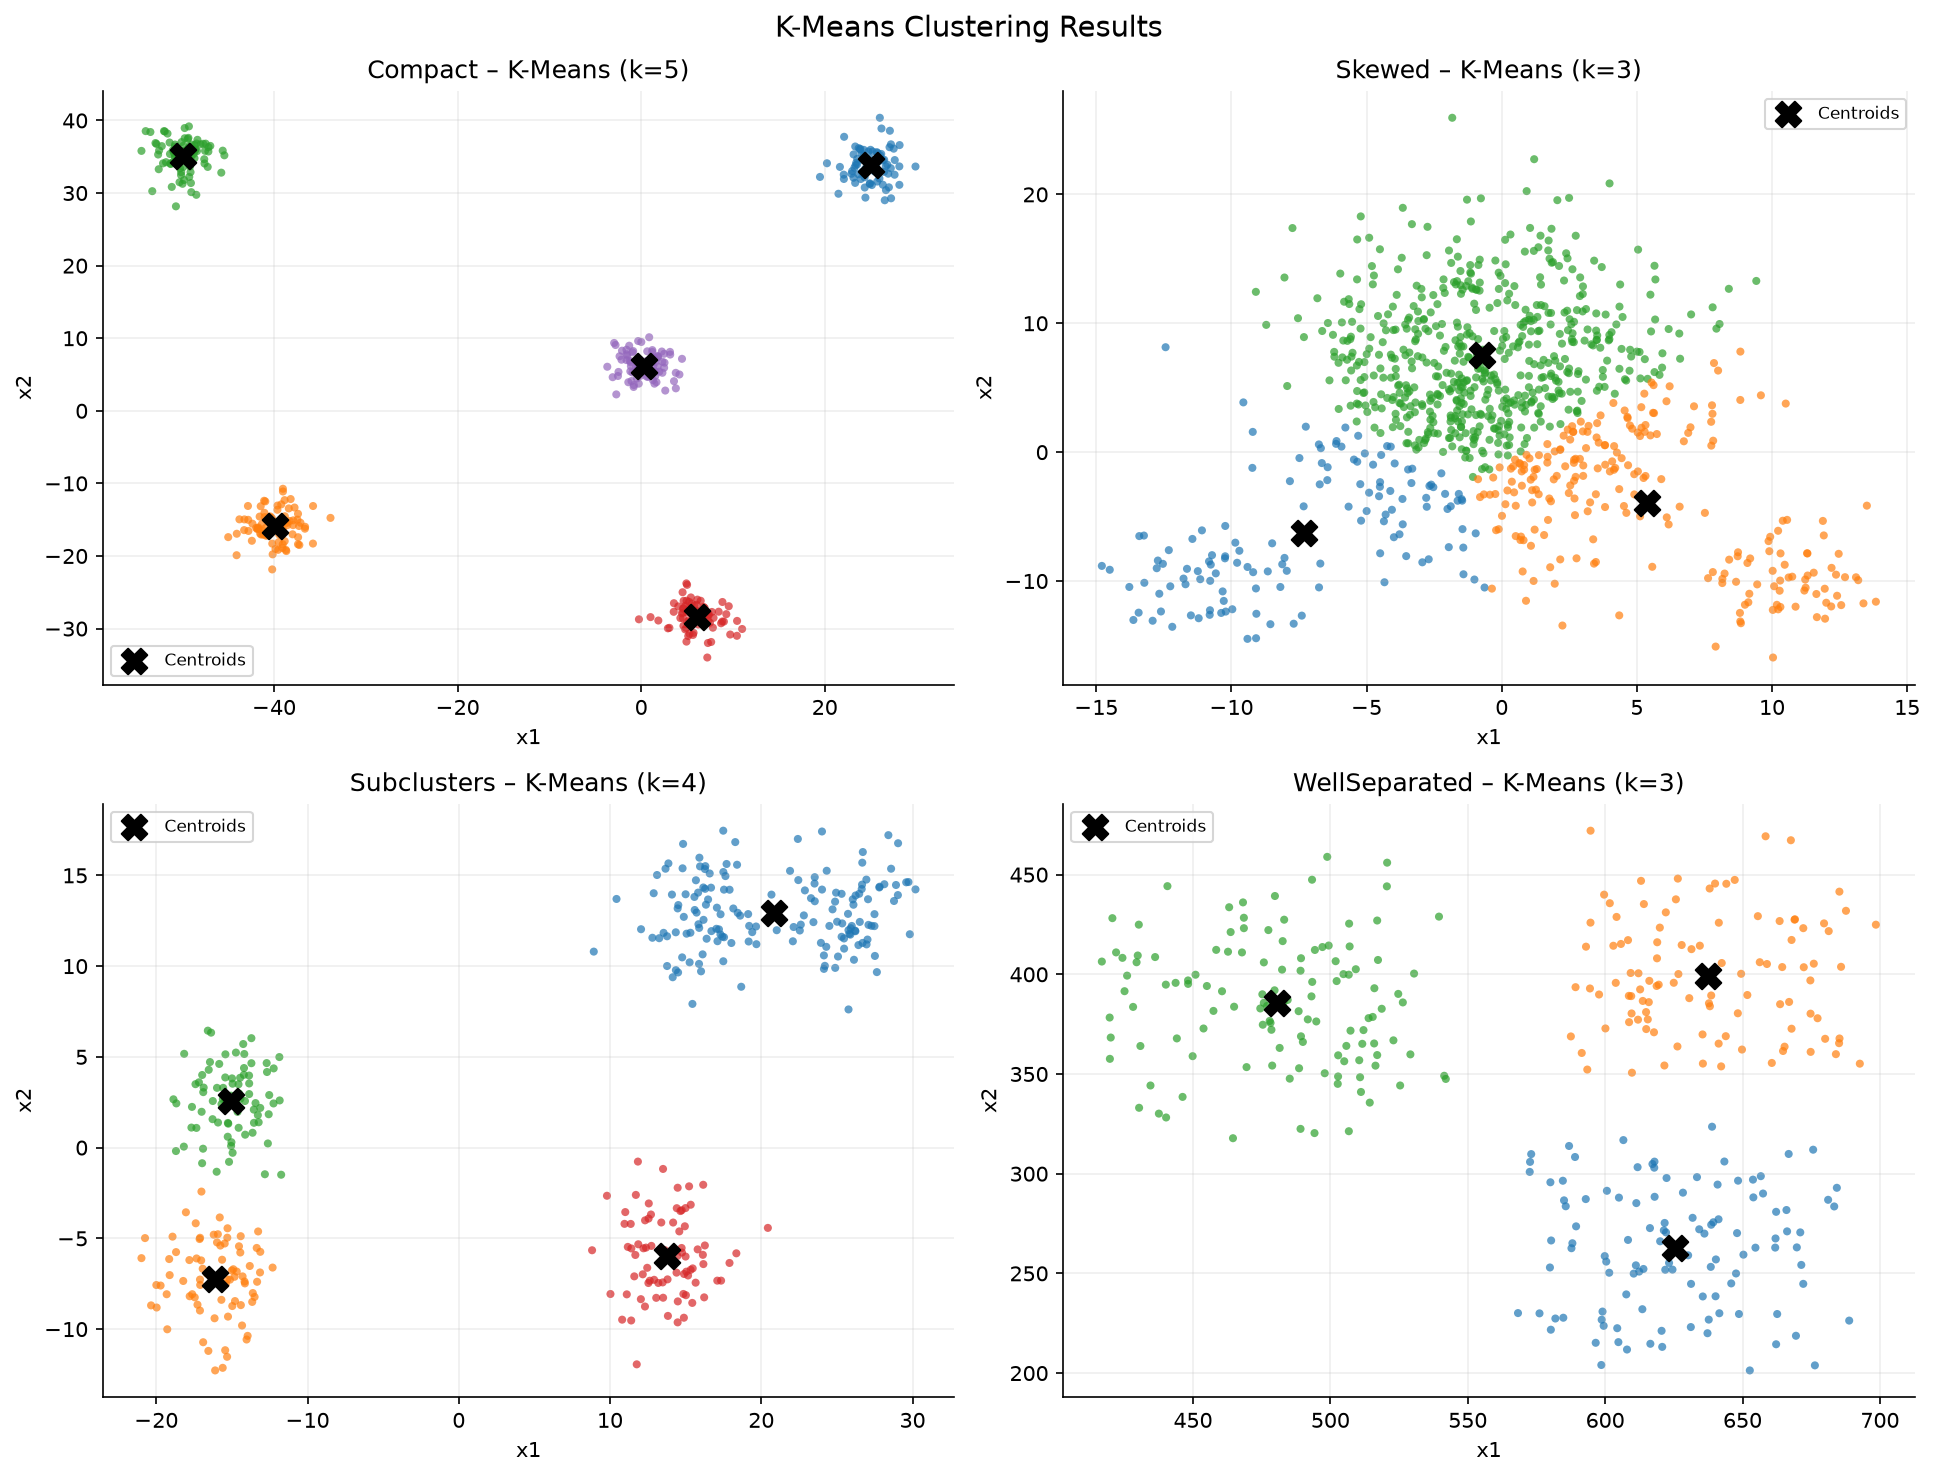
\includegraphics[width=0.62\textwidth]{part3_kmeans_results.png}
\caption{K-Means clusters at the silhouette-optimal $k$ (5, 3, 4, 3).}
\end{figure}

\subsection{Agglomerative clustering}
Single, complete, average and Ward linkage were compared; Fig.~\ref{fig:dendro} shows the Ward
dendrograms (last 40 merges) cut at the chosen $k$.
\begin{figure}[H]\centering
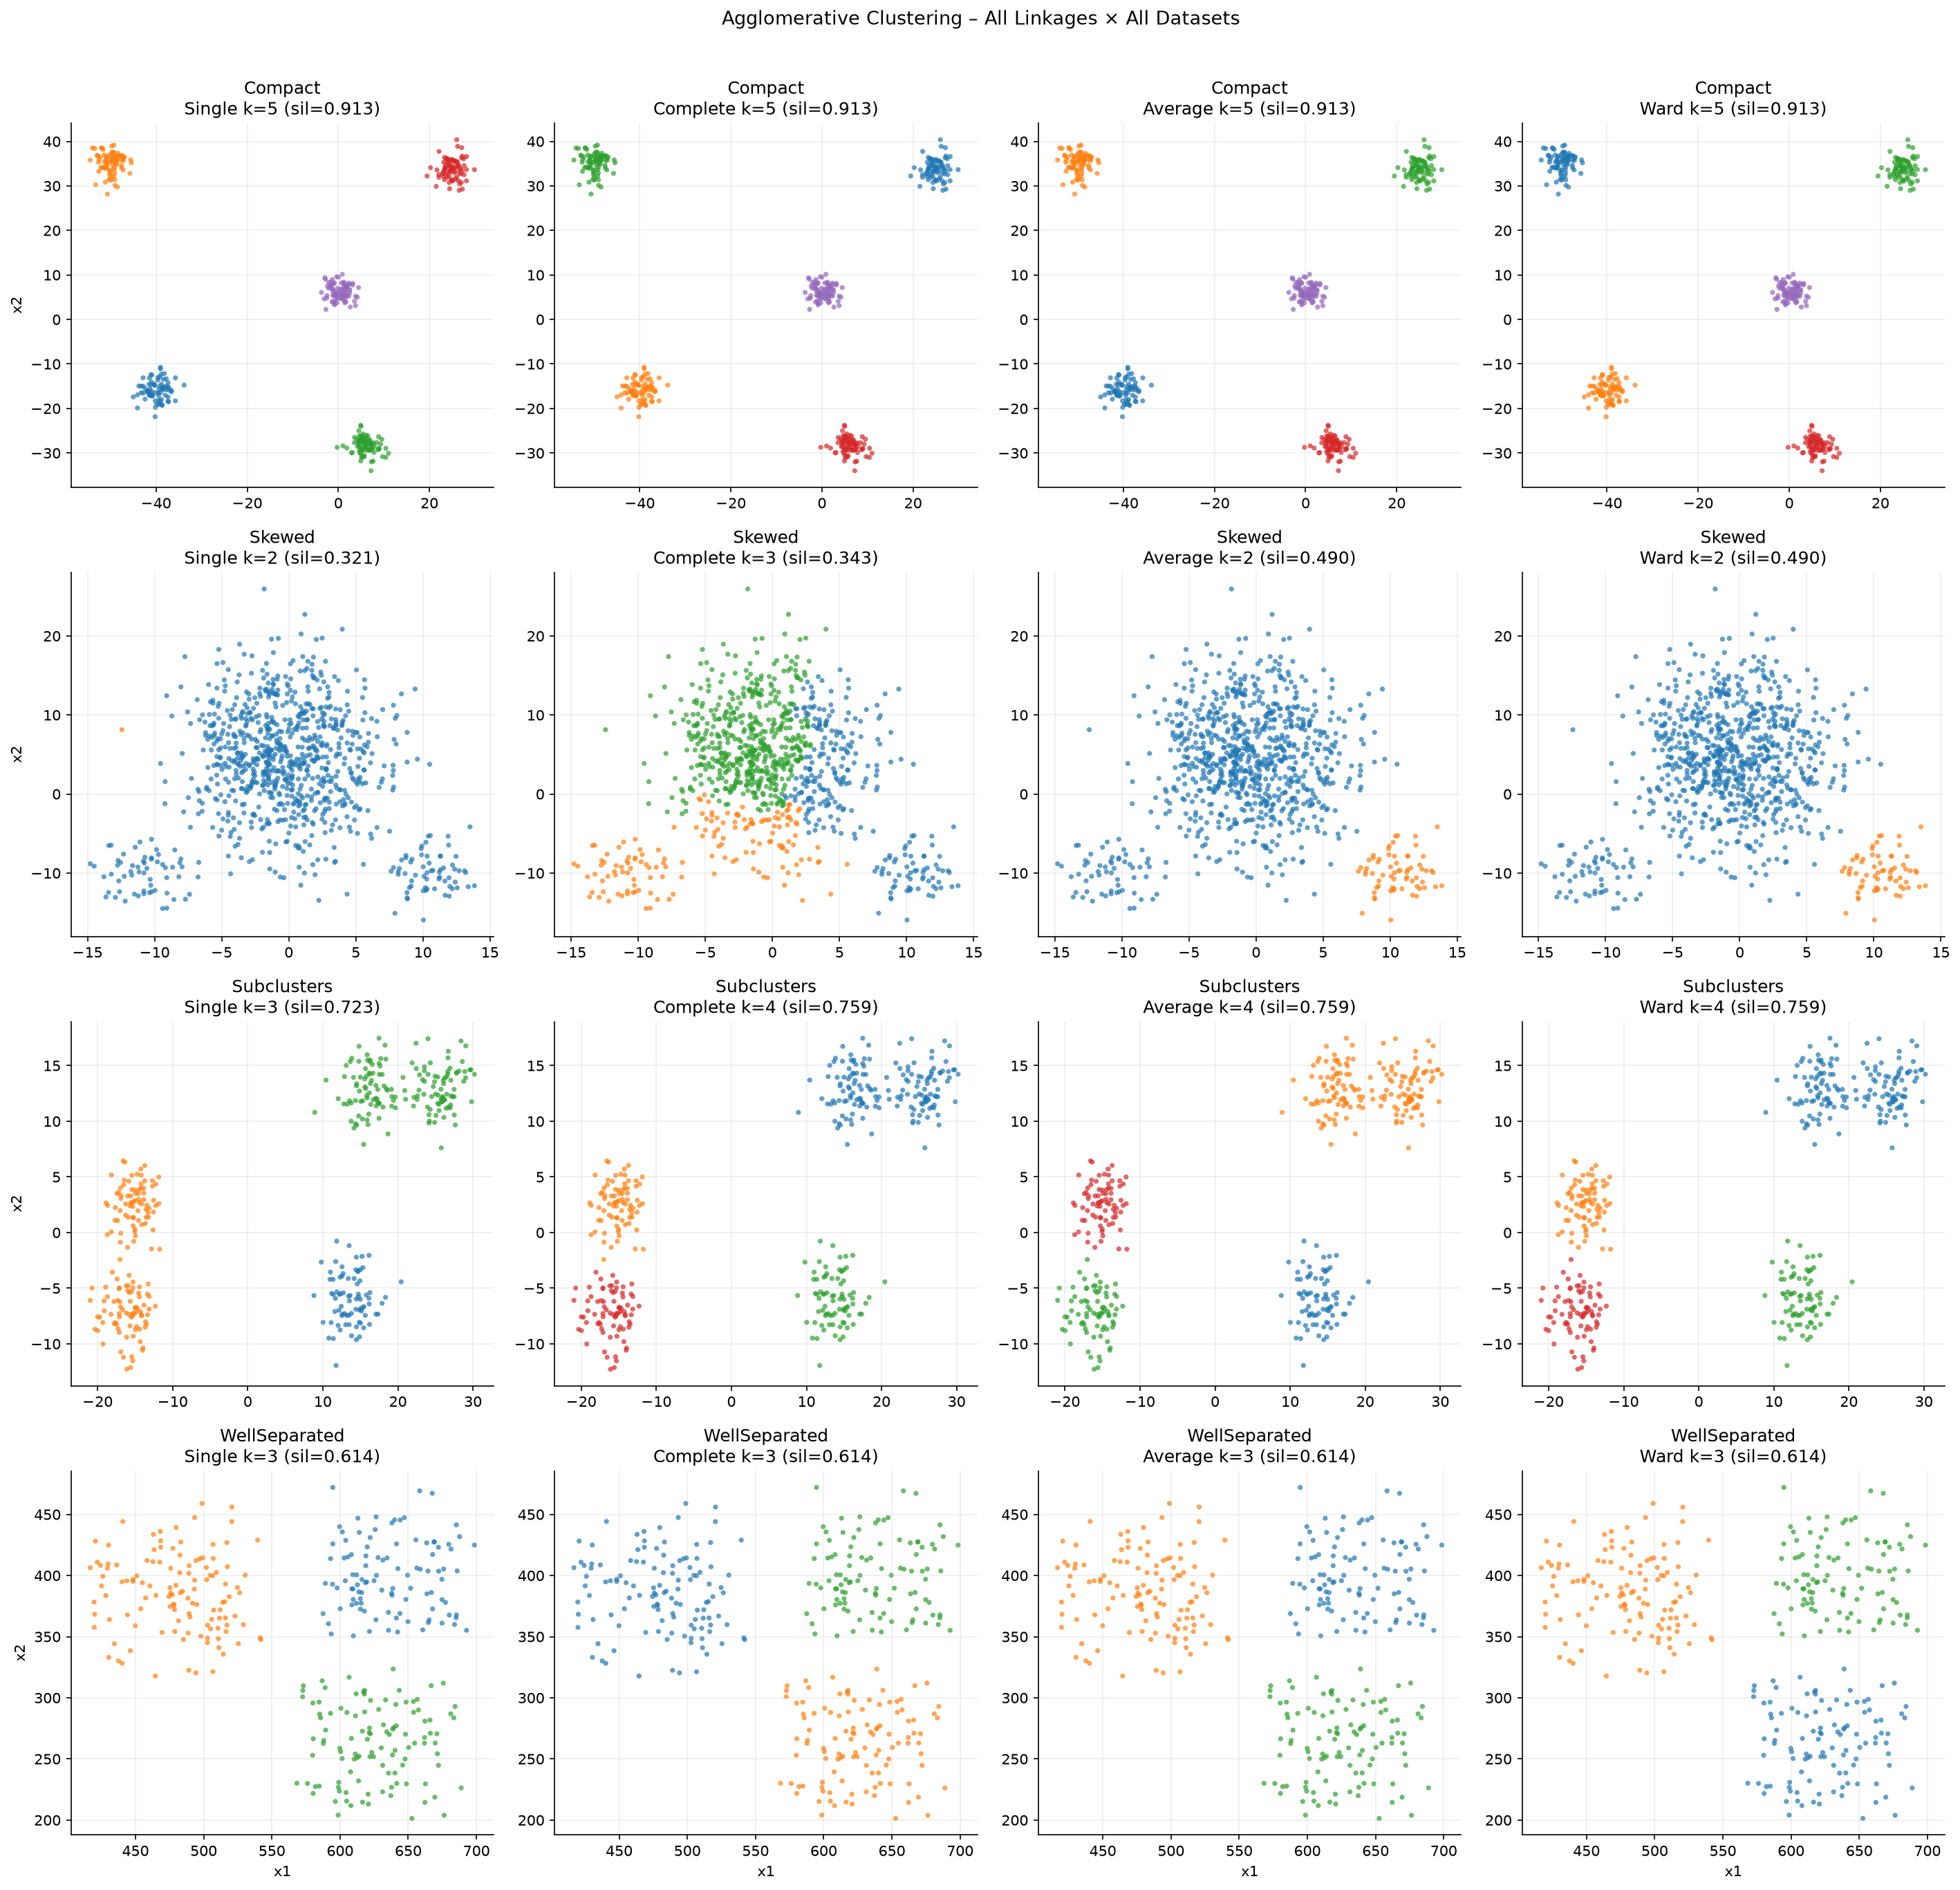
\includegraphics[width=0.75\textwidth]{part3_agglomerative_results.png}
\caption{Agglomerative clusters for all four linkages (rows: datasets).}
\end{figure}
\begin{figure}[H]\centering
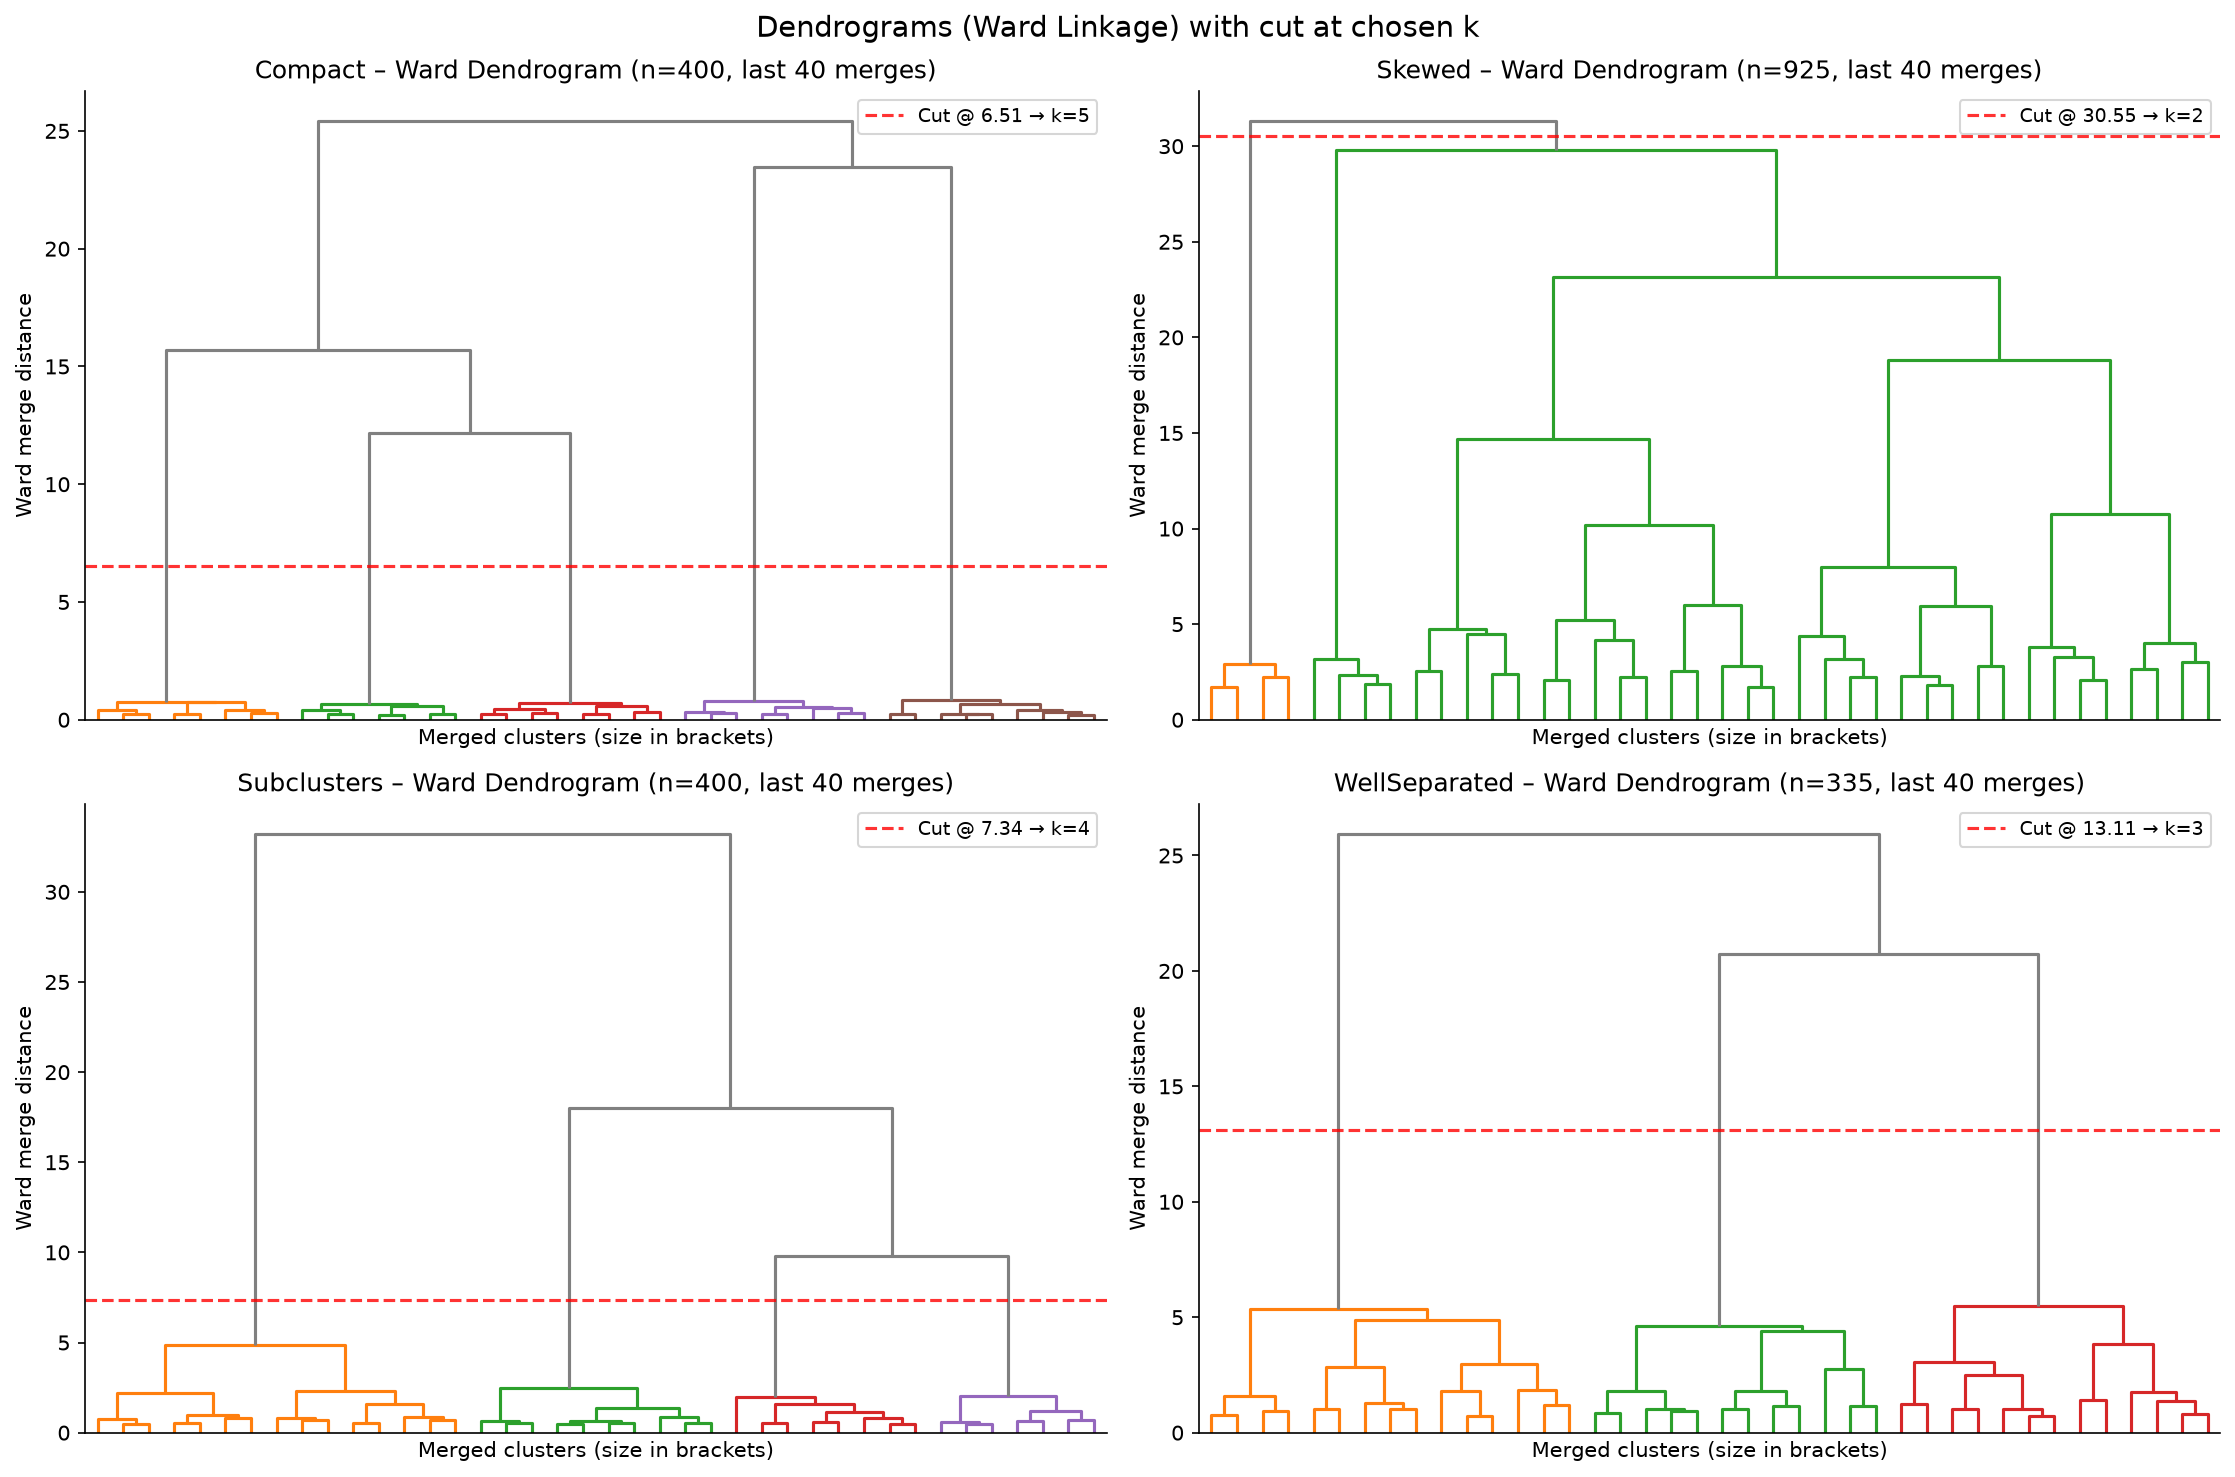
\includegraphics[width=0.75\textwidth]{part3_dendrograms.png}
\caption{Ward dendrograms with the cut (red) at the chosen $k$.}\label{fig:dendro}
\end{figure}
The Compact cut (6.51) lies in a huge gap (merge heights 0.86 $\to$ 12.17), WellSeparated
(13.11) in a clear gap (5.47 $\to$ 20.75). For Subclusters the merge at 4.87 just below the cut
(7.34) is the fusion of the two top-right sub-clusters. For Skewed the $k=2$ cut (30.55) lies
between 29.78 and 31.32: there is no well-defined level in the hierarchy.

\subsection{DBSCAN}
\texttt{min\_samples} (minPts) = 4 ($=2D$ for 2-D data, Ester et al.\ / Sander et al.): small enough not to
erode the borders of small clusters (50--600 points each), large enough to reject isolated points.
\texttt{eps} is the knee of the sorted 4-distance curve, found with the maximum-perpendicular-distance
(chord) heuristic, re-applied to the tail right of the first knee: on clean blobs the first knee
(83--91st percentile) was too early and labelled 5--10\% of points as noise; the refined knee lies
at the 96--99th percentile.
\begin{figure}[H]\centering
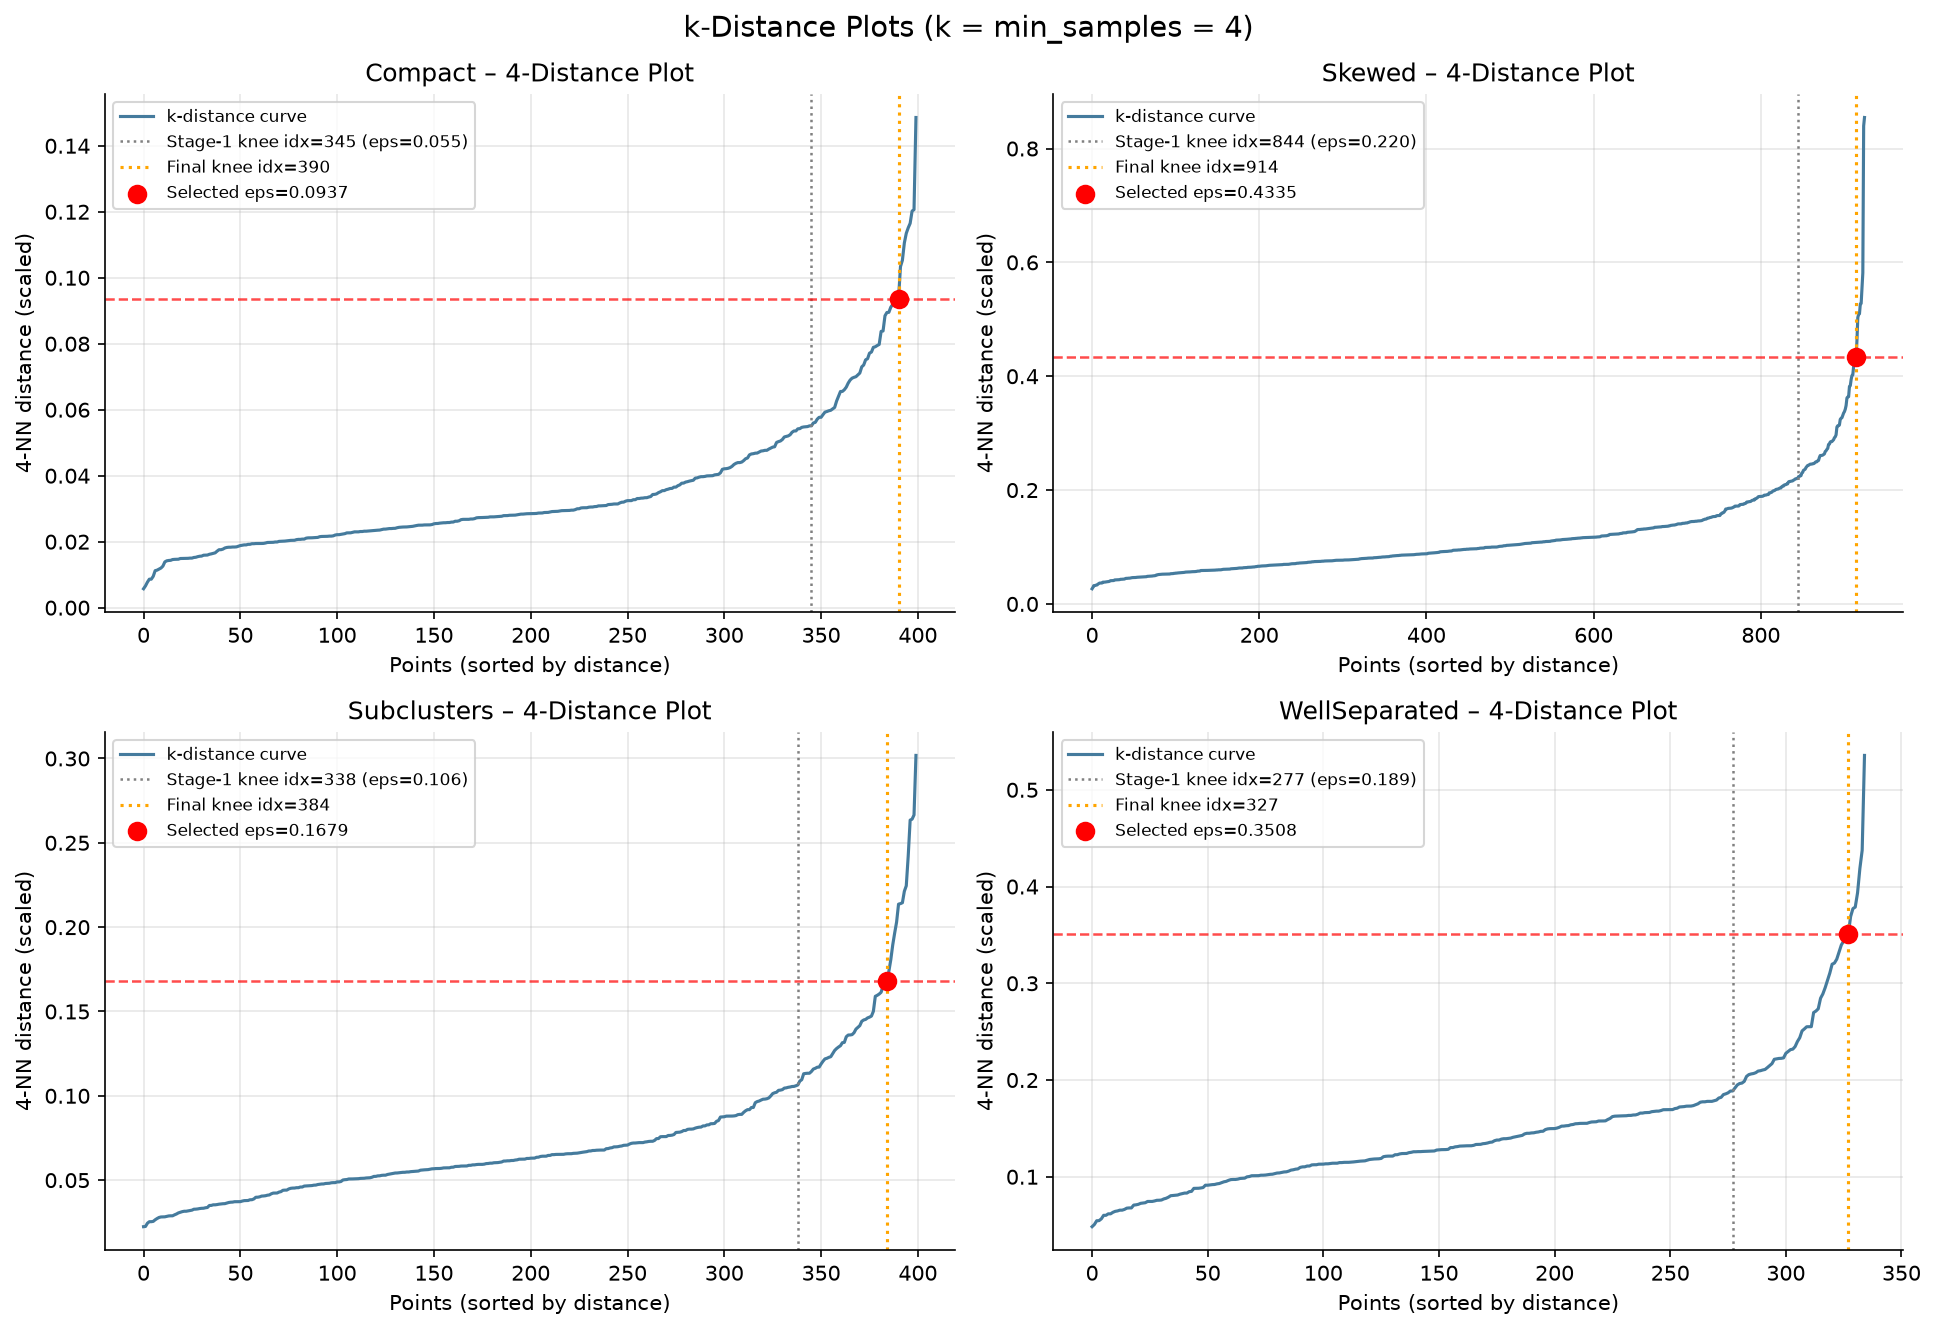
\includegraphics[width=0.6\textwidth]{part3_kdistance_plots.png}
\caption{Sorted 4-distance plots with the chosen eps.}
\end{figure}
\begin{figure}[H]\centering
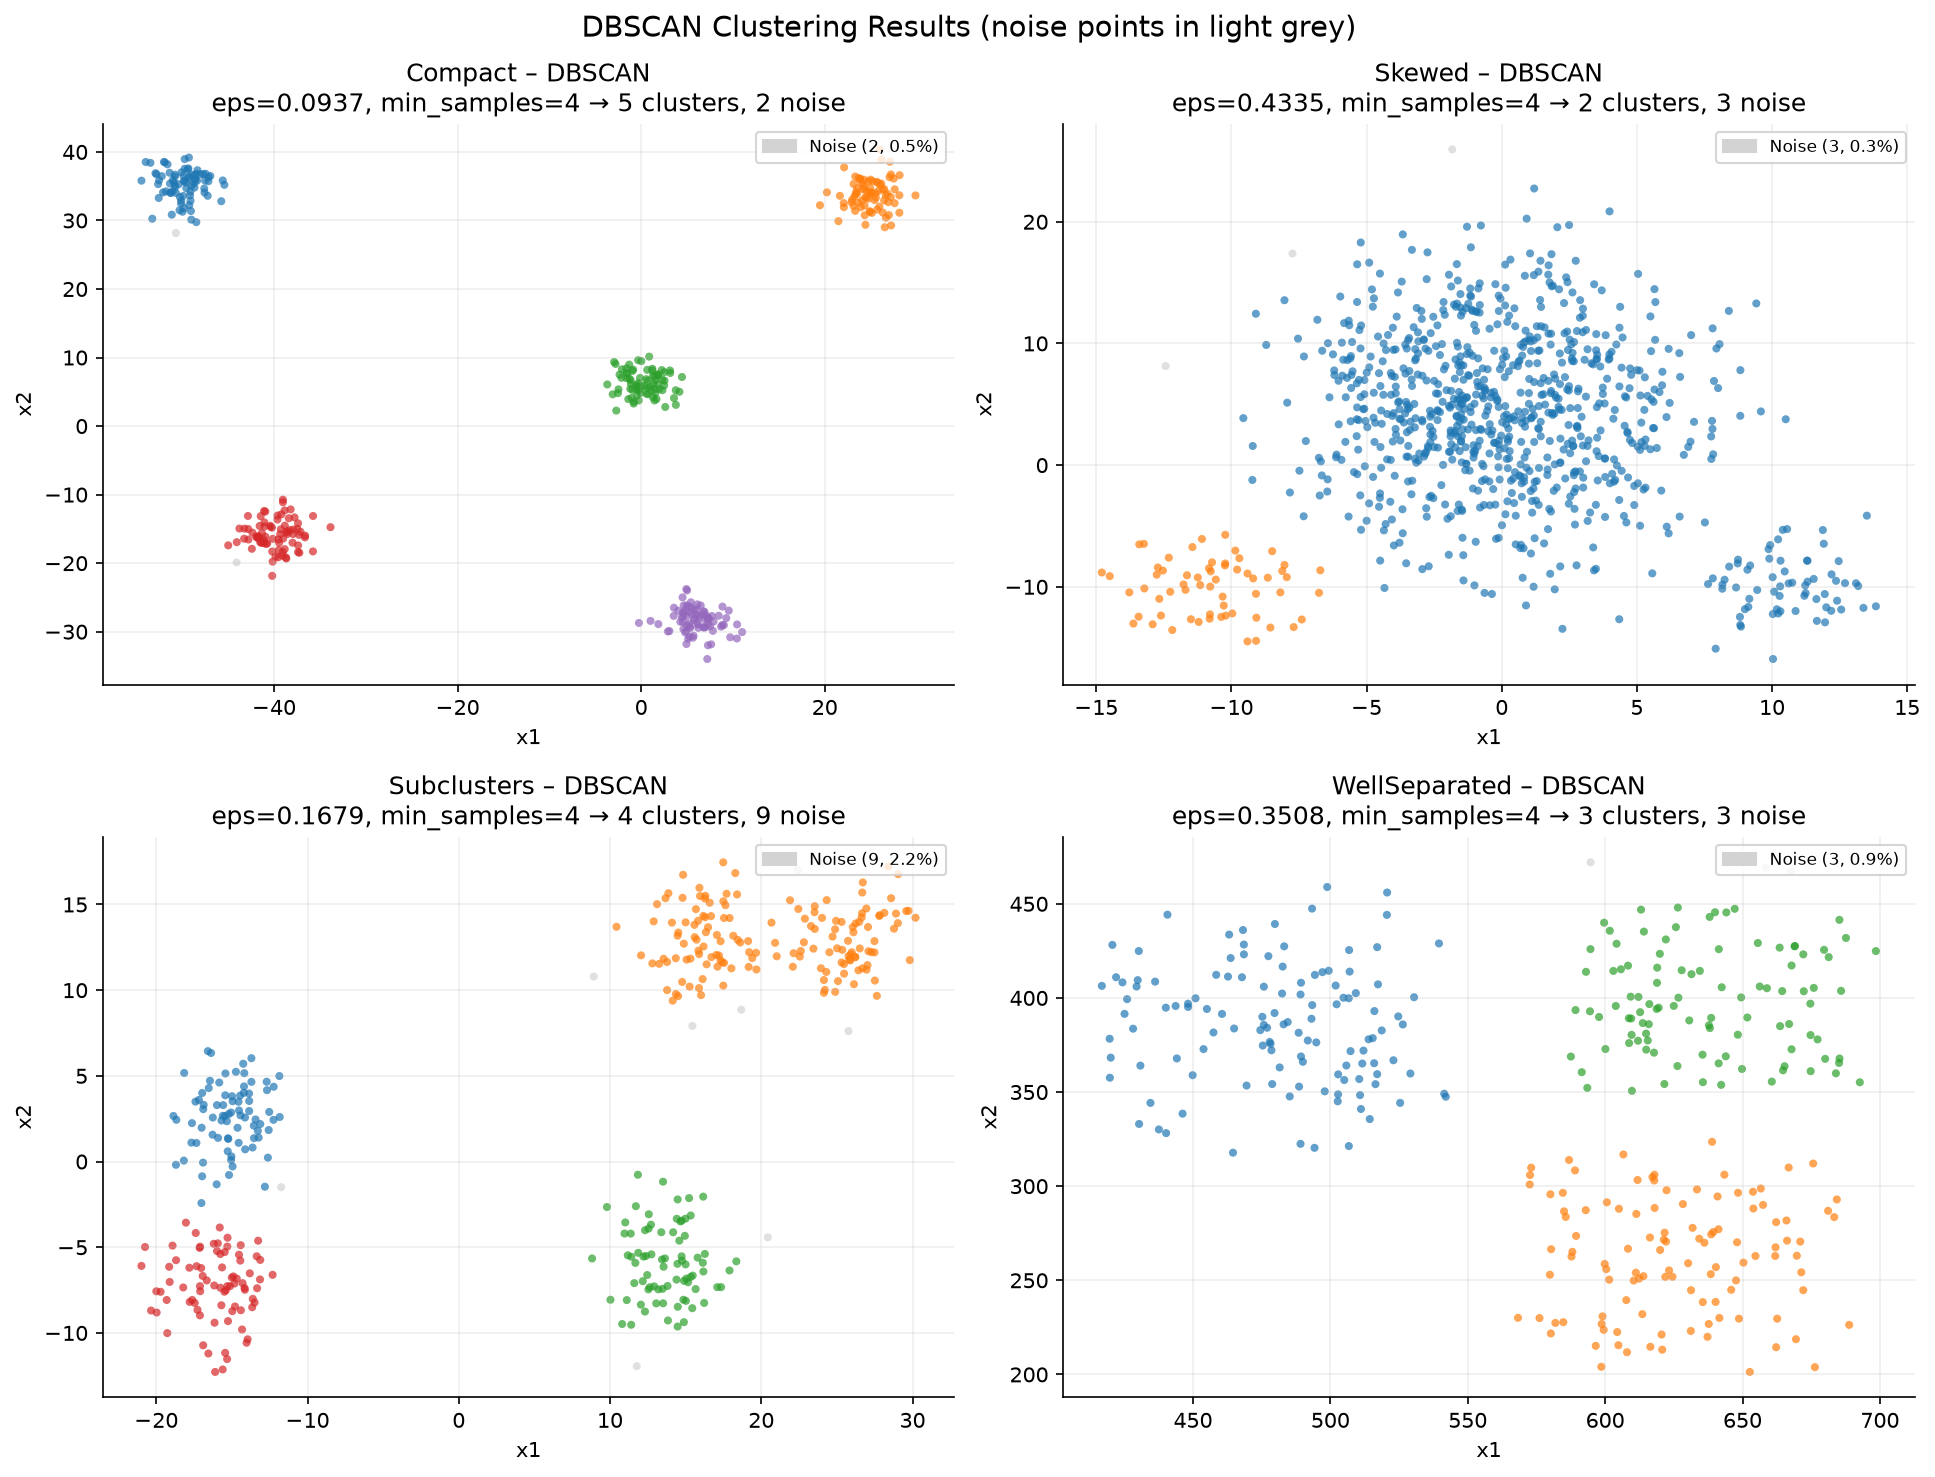
\includegraphics[width=0.62\textwidth]{part3_dbscan_results.png}
\caption{DBSCAN clusters (noise in grey).}
\end{figure}

A sensitivity run ($0.8$--$1.2\times$eps) shows stable cluster counts for Compact (always 5) and
WellSeparated (always 3). For Subclusters, 4 clusters up to $1.0\times$ and 3 from $1.1\times$. For
Skewed eps is critical: $0.8\times$ and $0.9\times$ (0.347/0.390) give the true 3 groups with 11/6
noise points, $1.0\times$ gives 2, $1.1\times$ a single cluster.

\subsection{Parameters and scores}
\begin{table}[H]\centering\small
\caption{Parameters used.}\label{tab:params}\setlength{\tabcolsep}{4pt}
\begin{tabular}{@{}lccccccc@{}}\toprule
Dataset & K-Means $k$ & Agglo $k$ (S/C/A/W) & Ward cut & eps & minPts & DBSCAN $k$ & Noise\\\midrule
Compact & 5 & 5/5/5/5 & 6.51 & 0.0937 & 4 & 5 & 2 (0.5\%)\\
Skewed & 3 & 2/3/2/2 & 30.55 & 0.4335 & 4 & 2 & 3 (0.3\%)\\
Subclusters & 4 & 3/4/4/4 & 7.34 & 0.1679 & 4 & 4 & 9 (2.2\%)\\
WellSeparated & 3 & 3/3/3/3 & 13.11 & 0.3508 & 4 & 3 & 3 (0.9\%)\\\bottomrule
\end{tabular}\end{table}

\begin{table}[H]\centering\small
\caption{Internal scores (Sil.\ $\uparrow$, DB $\downarrow$, CH $\uparrow$). DBSCAN scores exclude noise. Bold: best per dataset.}\label{tab:scores}
\begin{tabular}{@{}llrrrrr@{}}\toprule
Dataset & Algorithm ($k$) & Sil. & DB & CH & Noise & \%\\\midrule
Compact & K-Means / all 4 linkages (5) & 0.9133 & 0.1183 & 18{,}056.99 & 0 & 0.0\\
 & DBSCAN (5) & \textbf{0.9139} & \textbf{0.1178} & \textbf{18{,}368.03} & 2 & 0.5\\\midrule
Skewed & K-Means (3) & 0.4093 & 0.8573 & \textbf{658.43} & 0 & 0.0\\
 & Agglo single (2) & 0.3206 & \textbf{0.4837} & 3.06 & 0 & 0.0\\
 & Agglo complete (3) & 0.3434 & 1.0155 & 484.94 & 0 & 0.0\\
 & Agglo average (2) & \textbf{0.4897} & 0.5111 & 333.09 & 0 & 0.0\\
 & Agglo Ward (2) & \textbf{0.4897} & 0.5111 & 333.09 & 0 & 0.0\\
 & DBSCAN (2) & 0.4870 & 0.5358 & 302.94 & 3 & 0.3\\\midrule
Subclusters & K-Means (4) & 0.7590 & 0.3281 & 2{,}682.15 & 0 & 0.0\\
 & Agglo single (3) & 0.7226 & 0.4174 & 1{,}655.44 & 0 & 0.0\\
 & Agglo complete (4) & 0.7587 & 0.3287 & 2{,}679.99 & 0 & 0.0\\
 & Agglo average / Ward (4) & 0.7590 & 0.3281 & 2{,}682.15 & 0 & 0.0\\
 & DBSCAN (4) & \textbf{0.7648} & \textbf{0.3220} & \textbf{2{,}791.81} & 9 & 2.2\\\midrule
WellSeparated & K-Means / all 4 linkages (3) & 0.6137 & 0.5374 & 773.67 & 0 & 0.0\\
 & DBSCAN (3) & \textbf{0.6148} & \textbf{0.5313} & \textbf{780.34} & 3 & 0.9\\\bottomrule
\end{tabular}\end{table}

\subsection{Best algorithm per dataset}
\begin{itemize}
\item \textbf{Compact}: all methods tie; all find the five 80-point blobs. DBSCAN's marginally
better scores come only from dropping 2 boundary points.
\item \textbf{WellSeparated}: all methods tie (identical partition); DBSCAN again gains only by
excluding 3 outer points.
\item \textbf{Subclusters}: K-Means = average = Ward ($k=4$), complete practically equal, DBSCAN the
same 4 groups plus 9 noise points. All merge the two top-right sub-clusters; none recovers the
5-blob level at its chosen parameters. Single linkage ($k=3$) is worst: it chains the two left groups.
\item \textbf{Skewed}: no method recovers all three groups at its chosen parameters. Average/Ward
($k=2$, sil.\ 0.4897) isolate the bottom-right group but absorb the bottom-left one into the cloud;
DBSCAN (sil.\ 0.4870) does the mirror image. DBSCAN with $0.9\times$eps is the only configuration
that separates all three real groups, so it is the most capable method here, but fragile in eps.
\end{itemize}

\subsection{Why algorithms fail (by assumption)}
\begin{description}
\item[K-Means: shape, size, variance.] Assumes convex, isotropic clusters of similar size and
variance (Voronoi cells). On Skewed, with $k=3$ it splits the large high-variance cloud into wedges
and attaches each small group to one wedge, despite the right $k$ and the best CH (658.4).
\item[Single linkage: chaining.] Merges through the closest pair, so a thin bridge of points joins
clusters. On Skewed the second ``cluster'' at $k=2$ is one isolated point (CH 3.06---its low DB of
0.4837 is an artefact); on Subclusters it chains the two left groups.
\item[Complete linkage: size/variance.] Prefers clusters of similar diameter; on Skewed it cuts the
large cloud and joins part of it with the bottom-left group (worst DB, 1.0155).
\item[Average/Ward: size/variance.] Ward shares K-Means' variance objective. On Skewed, splitting
off the distant small group is cheap, separating the one touching the cloud is not, so $k=2$ wins.
\item[DBSCAN: density, single global eps.] One eps must serve all clusters. On Skewed the cloud is
sparse and nearly touches the bottom-right group; at eps 0.4335 a chain of core points connects
them. The window of good eps values is narrow because the gaps are comparable to the spacing inside
the sparse cloud.
\end{description}

\subsection{Metric pitfalls}
\paragraph{Sum of intra-cluster distances cannot compare different k.} Inertia decreases
monotonically with $k$ (elbow plots): an extra centre can only shorten each point's distance to its
nearest centre, and $k=n$ gives 0. Comparing Skewed average-linkage ($k=2$) with K-Means ($k=3$) by
inertia would always favour the method with more clusters regardless of quality. Silhouette, DB and
CH balance cohesion against separation (CH explicitly by its $(n-k)/(k-1)$ factor), so they are
comparable across $k$.

\paragraph{Silhouette favours convex but wrong solutions.} $s(i)=(b(i)-a(i))/\max(a(i),b(i))$ uses
Euclidean mean distances: elongated, curved or large-variance clusters have a large $a(i)$, whereas
compact Voronoi pieces keep it small. On Skewed, average/Ward $k=2$ (0.4897) beats K-Means $k=3$
(0.4093) although neither is right, and on Subclusters silhouette prefers 4 groups (0.759) over the
true 5-blob structure. It rewards compact separated convex pieces, not the true shape.

\paragraph{Ignoring DBSCAN noise inflates its scores.} Noise points are those far from dense regions,
i.e.\ exactly the points with the worst silhouette and largest spread. Excluding them improves every
metric for the \emph{same} partition: Compact 0.9133 $\to$ 0.9139 (CH 18{,}057 $\to$ 18{,}368; 2 points),
WellSeparated 0.6137 $\to$ 0.6148 (3 points), Subclusters 0.7590 $\to$ 0.7648 (CH 2{,}682 $\to$
2{,}792; 9 points). With the earlier too-small eps (26 noise points, 6.5\% on Compact) the silhouette
rose to 0.9207 and CH to 20{,}334 for the very same five clusters. A run labelling most points as
noise would look near-perfect. DBSCAN scores must therefore always be reported with the noise count.

%=====================================================================
\section{Reflection: PowerBI vs.\ Python}
%=====================================================================
\textbf{Visualisation.} PowerBI is clearly better for \emph{exploration by non-programmers and for
communication}: charts are built by drag-and-drop, and slicers, cross-filtering and DAX measures make
every visual react to a selection, so a manager can ask ``what about PhD customers in the 70--90k band?''
without new code. Python (matplotlib/seaborn) is better for \emph{analytical} graphics: silhouette
plots, dendrograms, k-distance curves and radar charts are a few lines of code but are not standard
PowerBI visuals, plots are exactly reproducible and versionable, and they sit next to the computation
that produced them. PowerBI's correlation heatmap, for example, required computing the matrix
outside the standard visuals, which is one line (\texttt{df.corr()}) in pandas.

\textbf{Preprocessing.} Power Query records every step in an \emph{Applied Steps} list, which makes
simple cleaning (type conversion, filtering rows, replacing values, adding columns) transparent and
easy to audit, and refreshes automatically when the source changes. It becomes awkward for anything
statistical: median imputation, outlier rules based on distributions, or scaling require M/DAX
workarounds, and the logic is hidden in a binary \texttt{.pbix} that cannot be diffed or reviewed in
git. In Python the same steps are explicit code, testable (we verified every Power Query step against
the raw file with pandas), and they integrate directly with modelling (scaling, clustering, tests).
Our workflow used each tool for its strength: PowerBI for cleaning plus an interactive report,
Python for clustering, validation and analytical plots.

%=====================================================================
\section{Conclusions}
%=====================================================================
\begin{itemize}
\item The PowerBI analysis showed that income ($r=0.79$ with spending), children ($r=-0.50$) and
web-visit intensity ($r=-0.50$) are the main axes of customer value; the K-Means segments recover
exactly these axes: affluent child-free big spenders (cluster 1), young low-income heavy browsers
(cluster 0), loyal deal-seeking families (cluster 2) and new low-spending families (cluster 3).
\item The response-rate patterns from Task 1 (higher for high income, no children and long tenure)
suggest that clusters 1 and 2 will be the most responsive---to be tested in Section 3, since campaign
variables were deliberately excluded from clustering.
\item Our from-scratch K-Means matches sklearn (inertia within 0.0014\%, ARI 1.0 from equal start).
$k=4$ was chosen from stability and business usability since elbow and silhouette were inconclusive;
the low silhouette (0.17) means the segments are useful summaries rather than natural, separated groups.
Education (weakly) but not Complain aligns with the segments.
\item On the synthetic data every algorithm succeeds when clusters are compact, similar and well
separated. Differences appear with unequal size/variance (Skewed): K-Means and Ward impose convex,
equal-variance pieces, single linkage chains, and only DBSCAN can recover the structure, at the price
of a sensitive eps. Internal indices must be interpreted with care: they favour convex solutions,
cannot be replaced by inertia across $k$, and DBSCAN's scores must be read together with its noise share.
\end{itemize}
\end{document}
